\documentclass[spanish,a4paper]{article}

% Paquetes generales
\usepackage[utf8]{inputenc}%esto permite meter tildes sin el coso
\usepackage[spanish]{babel}
\usepackage{ifthen}
\usepackage{amssymb}
\usepackage{amsmath} 
\usepackage{multicol}
\usepackage[absolute]{textpos}
\usepackage{hyperref}
%\usepackage{graphicx}
\usepackage{aed2-tad, aed2-symb, aed2-itef}
\usepackage{algpseudocode}
\usepackage{modulos}
\usepackage{caratula}
\usepackage{float}%este es el que acomoda bien las figures
\usepackage{tikz}
\usetikzlibrary{calc}
\pgfdeclarelayer{bg}
\pgfsetlayers{bg,main}
%==========================
\usepackage[Pseudocodigo]{algorithm}
\usepackage{algorithmicx}
\usepackage[latin1]{inputenc} %Codificacion iso-8889-1
\usepackage{tikz}
\usetikzlibrary{arrows,positioning, calc} 
\tikzstyle{vertex}=[draw,fill=black!15,circle,minimum size=18pt,inner sep=0pt]
%==========================
\usepackage{listings}
\usepackage{color}



%New colors defined belowe Holi
\definecolor{codegreen}{rgb}{0,0.6,0}
\definecolor{codegray}{rgb}{0.5,0.5,0.5}
\definecolor{codepurple}{rgb}{0.58,0,0.82}
\definecolor{backcolour}{rgb}{0.95,0.95,0.92}

%Code listing style named "mystyle"
\lstdefinestyle{mystyle}{
  backgroundcolor=\color{backcolour},   commentstyle=\color{codegreen},
  keywordstyle=\color{magenta},
  numberstyle=\tiny\color{codegray},
  stringstyle=\color{codepurple},
  basicstyle=\footnotesize,
  breakatwhitespace=false,         
  breaklines=true,                 
  captionpos=b,                    
  keepspaces=true,                 
  numbers=left,                    
  numbersep=5pt,                  
  showspaces=false,                
  showstringspaces=false,
  showtabs=false,                  
  tabsize=2
}

%"mystyle" code listing set
\lstset{style=mystyle}

\newcommand{\linea}{\noindent\rule{15cm}{0.4pt}}
\newcommand{\ode}[1]{\begin{flushright} $\mathcal{O}(#1)$ \end{flushright}}

%% **************************************************************************
%
%  Package 'caratula', version 0.5 (para componer caratulas de TPs del DC).
%
%  En caso de dudas, problemas o sugerencias sobre este package escribir a
%  Brian J. Cardiff (bcardif arroba gmail.com).
%  Nico Rosner (nrosner arroba dc.uba.ar).
%
% **************************************************************************

% ----- Informacion sobre el package para el sistema -----------------------

\NeedsTeXFormat{LaTeX2e}
\ProvidesPackage{caratula}[2013/08/04 v0.5 Para componer caratulas de TPs del DC]
\RequirePackage{ifthen}
\usepackage[pdftex]{graphicx}

% ----- Imprimir un mensajito al procesar un .tex que use este package -----

\typeout{Cargando package 'caratula' v0.5 (2013/08/04)}

% ----- Algunas variables --------------------------------------------------

\let\Materia\relax
\let\Submateria\relax
\let\Titulo\relax
\let\Subtitulo\relax
\let\Grupo\relax
\let\Fecha\relax
\let\Logoimagefile\relax
\newcommand{\LabelIntegrantes}{}
\newboolean{showLU}
\newboolean{showEntregas}
\newboolean{showDirectores}

% ----- Comandos para que el usuario defina las variables ------------------

\def\materia#1{\def\Materia{#1}}
\def\submateria#1{\def\Submateria{#1}}
\def\titulo#1{\def\Titulo{#1}}
\def\subtitulo#1{\def\Subtitulo{#1}}
\def\grupo#1{\def\Grupo{#1}}
\def\fecha#1{\def\Fecha{#1}}
\def\logoimagefile#1{\def\Logoimagefile{#1}}

% ----- Token list para los integrantes ------------------------------------

\newtoks\intlist\intlist={}

\newtoks\intlistSinLU\intlistSinLU={}

\newcounter{integrantesCount}
\setcounter{integrantesCount}{0}
\newtoks\intTabNombre\intTabNombre={}
\newtoks\intTabLU\intTabLU={}
\newtoks\intTabEmail\intTabEmail={}

\newcounter{directoresCount}
\setcounter{directoresCount}{0}
\newtoks\direcTabNombre\direcTabNombre={}
\newtoks\direcTabEmail\direcTabEmail={}

% ----- Comando para que el usuario agregue integrantes --------------------

\def\integrante#1#2#3{%
    \intlist=\expandafter{\the\intlist\rule{0pt}{1.2em}#1&#2&\tt #3\\[0.2em]}%
    \intlistSinLU=\expandafter{\the\intlistSinLU\rule{0pt}{1.2em}#1 & \tt #3\\[0.2em]}%
    %
    \ifthenelse{\value{integrantesCount} > 0}{%
        \intTabNombre=\expandafter{\the\intTabNombre & #1}%
        \intTabLU=\expandafter{\the\intTabLU & #2}%
        \intTabEmail=\expandafter{\the\intTabEmail & \tt #3}%
    }{
        \intTabNombre=\expandafter{\the\intTabNombre #1}%
        \intTabLU=\expandafter{\the\intTabLU #2}%
        \intTabEmail=\expandafter{\the\intTabEmail \tt #3}%
    }%
    \addtocounter{integrantesCount}{1}%
}

\def\director#1#2{%
    \ifthenelse{\value{directoresCount} > 0}{%
        \direcTabNombre=\expandafter{\the\direcTabNombre & #1}%
        \direcTabEmail=\expandafter{\the\direcTabEmail & \tt #2}%
    }{
        \direcTabNombre=\expandafter{\the\direcTabNombre #1}%
        \direcTabEmail=\expandafter{\the\direcTabEmail \tt #2}%
    }%
    \addtocounter{directoresCount}{1}%
}

% ----- Macro para generar la tabla de integrantes -------------------------

\newcommand{\tablaIntegrantes}{\ }

\newcommand{\tablaIntegrantesVertical}{%
\ifthenelse{\boolean{showLU}}{%
    \begin{tabular}[t]{| l @{\hspace{4ex}} c @{\hspace{4ex}} l|}
        \hline
        \multicolumn{1}{|c}{\rule{0pt}{1.2em} \LabelIntegrantes} & LU &  \multicolumn{1}{c|}{Correo electr\'onico} \\[0.2em]
        \hline \hline
        \the\intlist
        \hline
    \end{tabular}
}{
    \begin{tabular}[t]{| l @{\hspace{4ex}} @{\hspace{4ex}} l|}
        \hline
        \multicolumn{1}{|c}{\rule{0pt}{1.2em} \LabelIntegrantes} &  \multicolumn{1}{c|}{Correo electr\'onico} \\[0.2em]
        \hline \hline
        \the\intlistSinLU
        \hline
    \end{tabular}
    }%
}

\newcommand{\tablaIntegrantesHorizontal}{%
    \begin{tabular}[t]{ *{\value{integrantesCount}}{c} }
    \the\intTabNombre \\%
\ifthenelse{\boolean{showLU}}{
    \the\intTabLU \\%
}{}
    \the\intTabEmail %
    \end{tabular}%
}

\newcommand{\tablaDirectores}{%
\ifthenelse{\boolean{showDirectores}}{%
	\bigskip
	Directores

	\smallskip
    \begin{tabular}[t]{ *{\value{directoresCount}}{c} }
    \the\direcTabNombre \\%
    \the\direcTabEmail %
    \end{tabular}%
}{}%
}

\newcommand{\tablaEntregas}{%
\ifthenelse{\boolean{showEntregas}}{%
  \bigskip%
  \begin{tabular}[t]{|l p{3.5cm} p{1.5cm}|}%
  \hline%
  \rule{0pt}{1.2em} Instancia & Docente & Nota \\[0.2em] %
  \hline%
  \hline%
  \rule{0pt}{1.2em} Primera entrega & & \\[0.2em] %
  \hline%
  \rule{0pt}{1.2em} Segunda entrega & & \\[0.2em] %
  \hline%
  \end{tabular}%
}{}%
}

% ----- Codigo para manejo de errores --------------------------------------

\def\se{\let\ifsetuperror\iftrue}
\def\ifsetuperror{%
    \let\ifsetuperror\iffalse
    \ifx\Materia\relax\se\errhelp={Te olvidaste de proveer una \materia{}.}\fi
    \ifx\Titulo\relax\se\errhelp={Te olvidaste de proveer un \titulo{}.}\fi
    \edef\mlist{\the\intlist}\ifx\mlist\empty\se%
    \errhelp={Tenes que proveer al menos un \integrante{nombre}{lu}{email}.}\fi
    \expandafter\ifsetuperror}

\def\aftermaketitle{%
  \setcounter{page}{1}
}

% ----- \maketitletxt correspondiente a la versi�n v0.2.1 (texto v0.2 + fecha ) ---------

\def\maketitletxt{%
    \ifsetuperror\errmessage{Faltan datos de la caratula! Ingresar 'h' para mas informacion.}\fi
    \thispagestyle{empty}
    \begin{center}
    \vspace*{\stretch{2}}
    {\LARGE\textbf{\Materia}}\\[1em]
    \ifx\Submateria\relax\else{\Large \Submateria}\\[0.5em]\fi
    \ifx\Fecha\relax\else{\Large \Fecha}\\[0.5em]\fi
    \par\vspace{\stretch{1}}
    {\large Departamento de Computaci\'on}\\[0.5em]
    {\large Facultad de Ciencias Exactas y Naturales}\\[0.5em]
    {\large Universidad de Buenos Aires}
    \par\vspace{\stretch{3}}
    {\Large \textbf{\Titulo}}\\[0.8em]
    {\Large \Subtitulo}
    \par\vspace{\stretch{3}}
    \ifx\Grupo\relax\else\textbf{\Grupo}\par\bigskip\fi
    \tablaIntegrantes
    \end{center}
    \vspace*{\stretch{3}}
    \newpage\aftermaketitle}

% ----- \maketitletxtlogo correspondiente v0.2.1 (texto con fecha y logo) ---------

\def\maketitletxtlogo{%
    \ifsetuperror\errmessage{Faltan datos de la caratula! Ingresar 'h' para mas informacion.}\fi
    \thispagestyle{empty}
    \begin{center}
    \ifx\Logoimagefile\relax\else\includegraphics{\Logoimagefile}\fi \hfill 
\includegraphics{logo_dc.jpg}\\[1em]
    \vspace*{\stretch{2}}
    {\LARGE\textbf{\Materia}}\\[1em]
    \ifx\Submateria\relax\else{\Large \Submateria}\\[0.5em]\fi
    \ifx\Fecha\relax\else{\large \Fecha}\\[0.5em]\fi
    \par\vspace{\stretch{1}}
    {\large Departamento de Computaci\'on}\\[0.5em]
    {\large Facultad de Ciencias Exactas y Naturales}\\[0.5em]
    {\large Universidad de Buenos Aires}
    \par\vspace{\stretch{3}}
    {\Large \textbf{\Titulo}}\\[0.8em]
    {\Large \Subtitulo}
    \par\vspace{\stretch{3}}
    \ifx\Grupo\relax\else\textbf{\Grupo}\par\bigskip\fi
    \tablaIntegrantes
    \end{center}
    \vspace*{\stretch{4}}
    \newpage\aftermaketitle}

% ----- \maketitlegraf correspondiente a la versi�n v0.3 (gr�fica) -------------

\def\maketitlegraf{%
    \ifsetuperror\errmessage{Faltan datos de la caratula! Ingresar 'h' para mas informacion.}\fi
%
    \thispagestyle{empty}

    \ifx\Logoimagefile\relax\else\includegraphics{\Logoimagefile}\fi \hfill 
\includegraphics{logo_dc.jpg}

    \vspace*{.06 \textheight}

    \noindent \textbf{\huge \Titulo}  \medskip \\
    \ifx\Subtitulo\relax\else\noindent\textbf{\large \Subtitulo} \\ \fi%
    \noindent \rule{\textwidth}{1 pt}

    {\noindent\large\Fecha \hspace*\fill \Materia} \\
    \ifx\Submateria\relax\else{\noindent \hspace*\fill \Submateria}\fi%

    \medskip%
    \begin{center}
        \ifx\Grupo\relax\else\textbf{\Grupo}\par\bigskip\fi
        \tablaIntegrantes

        \tablaDirectores

        \tablaEntregas
    \end{center}%
    \vfill%
%
    \begin{minipage}[t]{\textwidth}
        \begin{minipage}[t]{.55 \textwidth}
            
\includegraphics{logo_uba.jpg}
        \end{minipage}%%
        \begin{minipage}[b]{.45 \textwidth}
            \textbf{\textsf{Facultad de Ciencias Exactas y Naturales}} \\
            \textsf{Universidad de Buenos Aires} \\
            {\scriptsize %
            Ciudad Universitaria - (Pabell\'on I/Planta Baja) \\
                Intendente G\"uiraldes 2160 - C1428EGA \\
            Ciudad Aut\'onoma de Buenos Aires - Rep. Argentina \\
                Tel/Fax: (54 11) 4576-3359 \\
            http://www.fcen.uba.ar \\
            }
        \end{minipage}
    \end{minipage}%
%
    \newpage\aftermaketitle}

% ----- Reemplazamos el comando \maketitle de LaTeX con el nuestro ---------
\renewcommand{\maketitle}{\maketitlegraf}

% ----- Dependiendo de las opciones ---------
%
% opciones:
%   txt     : caratula solo texto.
%   txtlogo : caratula txt con logo del DC y del grupo (opcional).
%   graf    : (default) caratula grafica con logo del DC, UBA y del grupo (opcional).
%
\@makeother\*% some package redefined it as a letter (as color.sty)
%
% Layout general de la caratula
%
\DeclareOption{txt}{\renewcommand{\maketitle}{\maketitletxt}}
\DeclareOption{txtlogo}{\renewcommand{\maketitle}{\maketitletxtlogo}}
\DeclareOption{graf}{\renewcommand{\maketitle}{\maketitlegraf}}
%
% Etiqueta Autores o Integrantes
%
\DeclareOption{integrante}{\renewcommand{\LabelIntegrantes}{Integrante}}
\DeclareOption{autor}{\renewcommand{\LabelIntegrantes}{Autor}}
%
% Formato tabla de integrantes
%
\DeclareOption{intVert}{\renewcommand{\tablaIntegrantes}{\tablaIntegrantesVertical}}
\DeclareOption{intHoriz}{\renewcommand{\tablaIntegrantes}{\tablaIntegrantesHorizontal}}
\DeclareOption{conLU}{\setboolean{showLU}{true}}
\DeclareOption{sinLU}{\setboolean{showLU}{false}}
\DeclareOption{conEntregas}{\setboolean{showEntregas}{true}}
\DeclareOption{sinEntregas}{\setboolean{showEntregas}{false}}
\DeclareOption{showDirectores}{\setboolean{showDirectores}{true}}
\DeclareOption{hideDirectores}{\setboolean{showDirectores}{false}}
%
% Opciones predeterminadas
%
\ExecuteOptions{intVert}%
\ExecuteOptions{graf}%
\ExecuteOptions{integrante}%
\ExecuteOptions{conLU}%
\ExecuteOptions{hideDirectores}%
\ExecuteOptions{sinEntregas}%
%
\ProcessOptions\relax

\usepackage[margin=1in]{geometry}
\begin{document}


\titulo{Trabajo Pr\'{a}ctico}
\subtitulo{}

\fecha{\today}

\materia{Algoritmos y Estructuras de Datos 3}
\grupo{}

\integrante{Zavalla, Agustín}{670/13}{nkm747@gmail.com}
\integrante{Vázquez, Jésica}{318/13}{jesis\_93@hotmail.com}
\integrante{chiqui, El}{449/13}{mfosco2005@yahoo.com.ar}
\integrante{Fosco, Martín Esteban}{449/13}{mfosco2005@yahoo.com.ar}

\maketitle

\thispagestyle{empty}
\vspace{3cm}
\tableofcontents
\newpage
\vfill

\begin{abstract}
En este trabajo se implementaron algoritmos que proporcionen soluciones a los tres problemas recibidos. A continuación se realiza una descripción de estos, dando ejemplos, luego se describen en detalle los algoritmos que los resuelven, se explica por qué son correctos y se da una cota para la complejidad.
\end{abstract}

\newpage



\section{El Telégrafo}

\subsection{El Problema}

\subsubsection{Introducción}
Se plantea en este caso el problema de, dados:
\begin{itemize}

\item Una cantidad de kilómetros de cable para cada ramal.

\item Una cantidad $n$ de ciudades en un orden determinado, identificadas por la cantidad de kilómetros que las separan de la capital (además de la capital, que se encuentra implícita en el kilómetro $0$ en todas las sucesiones de ciudades propuestas).

\end{itemize}


Hallar la mayor cantidad posible de ciudades que se puedan conectar con dicho cable sin cortarlo, en otras palabras: optimizar el uso del cable para conectar la mayor cantidad de ciudades consecutivas de un ramal.
Como resultado del problema se quiere obtener cuántas ciudades se pudieron conectar para cada ramal.

Es necesario además que el algoritmo funcione con orden de complejidad O($n$).


\subsubsection{Ejemplos}

A modo de ejemplo de qué plantea el problema, y sus soluciones, se observan casos:\\ \\

\noindent\rule{13cm}{0.4pt}


Dados 3 km de cable y las siguientes ciudades: (identificadas por la cantidad de km que las separan de la capital).\\

\begin{figure}[H]
  \begin{tikzpicture}
    \hspace*{1.5cm}
    
    \node [fill=gray!30] (0) at (0,0) { 0 };
    \node [fill=gray!30] (2) at (1,0) { 1 };
    \node [fill=gray!30] (3) at (2,0) { 2 };
    \node [fill=gray!30] (6) at (6,0) { 6 };
    \node [fill=gray!30] (7) at (7,0) { 7 };
    \node [fill=gray!30] (10) at (10,0) { 10 };
    
    \begin{pgfonlayer}{bg}    % select the background layer
        \draw (0) (10);
    \end{pgfonlayer}
  
  \end{tikzpicture}
\end{figure}

En este caso, lo ideal sería conectar las ciudades 0, 1, 2 entre sí, ya que la cantidad de cable es suficiente y en total conseguiría conectar 3 ciudades, en otros lugares conseguiría conectar menos ciudades:\\

\begin{figure}[H]
  \begin{tikzpicture}
    \hspace*{1.5cm}
    
    \node [fill=gray!30] (0) at (0,0) { 0 };
    \node [fill=gray!30] (1) at (1,0) { 1 };
    \node [fill=gray!30] (2) at (2,0) { 2 };
    \node [fill=gray!30] (6) at (6,0) { 6 };
    \node [fill=gray!30] (7) at (7,0) { 7 };
    \node [fill=gray!30] (10) at (10,0) { 10 };
    
    \begin{pgfonlayer}{bg}    % select the background layer
        \hspace*{1.5cm}
        \draw (0)--(3) (10);
    \end{pgfonlayer}
  
  \end{tikzpicture}
\end{figure}

Nota: \textbf{NO} se pueden conectar las ciudades 0-2 y las 6-7 de la siguiente manera:

\begin{figure}[H]
  \begin{tikzpicture}
    \hspace*{1.5cm}
    
    \node [fill=gray!30] (0) at (0,0) { 0 };
    \node [fill=gray!30] (1) at (1,0) { 1 };
    \node [fill=gray!30] (2) at (2,0) { 2 };
    \node [fill=gray!30] (6) at (6,0) { 6 };
    \node [fill=gray!30] (7) at (7,0) { 7 };
    \node [fill=gray!30] (10) at (10,0) { 10 };
    
    \begin{pgfonlayer}{bg}    % select the background layer
        \hspace*{1.5cm}
        \draw (0)--(3) (6)--(7) (10);
    \end{pgfonlayer}
  
  \end{tikzpicture}
\end{figure}

Si bien se pueden conseguir 5 ciudades de esta manera, los intervalos no son consecutivos, sino que están separados, es necesario que sea distribuido en sólo un intervalo (dado que no se puede cortar el cable).

\newpage

\linea


Dados 10 km de cable y las siguientes ciudades: \\

\begin{figure}[H]
  \begin{tikzpicture}
    \hspace*{0.5cm}
    \node [fill=gray!30] (0) at (0,0) { 0 };
    \node [fill=gray!30] (2) at (1,0) { 2 };
    \node [fill=gray!30] (6) at (3,0) { 6 };
    \node [fill=gray!30] (8) at (4,0) { 8 };
    \node [fill=gray!30] (14) at (7,0) { 14 };
    \node [fill=gray!30] (16) at (8,0) { 16 };
    \node [fill=gray!30] (20) at (10,0) { 20 };
    \node [fill=gray!30] (22) at (11,0) { 22 };
    
    \begin{pgfonlayer}{bg}    % select the background layer
        \draw (0) (22);
    \end{pgfonlayer}
  \end{tikzpicture}
\end{figure}

En este caso existen varias respuestas posibles, todas con el mismo resultado, se pueden conseguir 4 ciudades como máximo de las siguientes maneras:

\begin{figure}[H]
  \begin{tikzpicture}
    \hspace*{0.5cm}
    \node [fill=gray!30] (0) at (0,0) { 0 };
    \node [fill=gray!30] (2) at (1,0) { 2 };
    \node [fill=gray!30] (6) at (3,0) { 6 };
    \node [fill=gray!30] (8) at (4,0) { 8 };
    \node [fill=gray!30] (14) at (7,0) { 14 };
    \node [fill=gray!30] (16) at (8,0) { 16 };
    \node [fill=gray!30] (20) at (10,0) { 20 };
    \node [fill=gray!30] (22) at (11,0) { 22 };
    
    \begin{pgfonlayer}{bg}    % select the background layer
        \hspace*{0.5cm}
        \draw (0)--(8) (22);
    \end{pgfonlayer}
  \end{tikzpicture}
\end{figure}

\begin{figure}[H]
  \begin{tikzpicture}
    \hspace*{0.5cm}
    \node [fill=gray!30] (0) at (0,0) { 0 };
    \node [fill=gray!30] (2) at (1,0) { 2 };
    \node [fill=gray!30] (6) at (3,0) { 6 };
    \node [fill=gray!30] (8) at (4,0) { 8 };
    \node [fill=gray!30] (14) at (7,0) { 14 };
    \node [fill=gray!30] (16) at (8,0) { 16 };
    \node [fill=gray!30] (20) at (10,0) { 20 };
    \node [fill=gray!30] (22) at (11,0) { 22 };
    
    \begin{pgfonlayer}{bg}    % select the background layer
        \hspace*{0.5cm}
        \draw (0) (6)--(16) (22);
    \end{pgfonlayer}
  \end{tikzpicture}
\end{figure}

\begin{figure}[H]
  \begin{tikzpicture}
    \hspace*{0.5cm}
    \node [fill=gray!30] (0) at (0,0) { 0 };
    \node [fill=gray!30] (2) at (1,0) { 2 };
    \node [fill=gray!30] (6) at (3,0) { 6 };
    \node [fill=gray!30] (8) at (4,0) { 8 };
    \node [fill=gray!30] (14) at (7,0) { 14 };
    \node [fill=gray!30] (16) at (8,0) { 16 };
    \node [fill=gray!30] (20) at (10,0) { 20 };
    \node [fill=gray!30] (22) at (11,0) { 22 };
    
    \begin{pgfonlayer}{bg}    % select the background layer
        \hspace*{0.5cm}
        \draw (0) (14)--(22);
    \end{pgfonlayer}
  \end{tikzpicture}
\end{figure}

Como el algoritmo debe retornar sólo el máximo de ciudades, cualquiera de los intervalos que tomemos para conectar con nuestros cables servirán a nuestro propósito.

En definitiva, la respuesta será 4 ciudades.

\linea

\subsection{El Algoritmo}
\subsubsection{Explicación}
Ahora, habiendo ya explicado el problema planteado y qué clase de resultados se esperan, se puede pasar a mostrar el algoritmo creado.

Se buscó para la resolución definir cómo debían observarse los datos de entrada para poder mantener tanto la eficacia como la eficiencia temporal.

Se pueden sacar ciertas observaciones de los datos recibidos:

\begin{itemize}

\item La lista de distancias de ciudades recibida puede ser recorrida un número constante "k" de veces, por lo que intentar organizar los datos de alguna manera más compleja que como son recibidos no parece ser necesario ni útil.

\item Como los cables que deben ser puestos deben formar un intervalo continuo, sin interrupciones, pareciera que la distancia que realmente importa en nuestra lista es aquella $relativa$: entre una ciudad y las adyacentes a ésta.


\item Este punto es una inferencia del anterior: pareciera más útil armar una segunda lista que tenga las distancias entre cada ciudad consecutiva para procesar los datos, contando en complejidad el armado de esta lista  como una recorrida más de la lista.

\end{itemize}

Luego de haber extraído estas ideas, se ideó un algoritmo goloso que cumple con todos los requisitos e intenta armar el intervalo más grande posible recorriendo toda la lista de ciudades y siguiendo estas premisas con cada iteración:

\begin{itemize}

\item Si puedo incorporar la ciudad siguiente a mi intervalo, la incorporo.

\item Si no puedo, guardo la cantidad de ciudades del intervalo ya armado (si es mayor a la cantidad ya guardada) y luego suelto la cantidad de ciudades necesarias para poder incorporar la que está siendo analizada al intervalo.

\item Si llegué al final de la lista de ciudades, me fijo cuál fué el intervalo más grande que pude armar y devuelvo la cantidad de ciudades que lo componen como resultado.
\end{itemize}

\newpage

Primero, generamos el array con las distancias entre cada ciudad $D$ (a diferencia de las distancias con la capital) y además declaramos dos acumuladores y los índices $i, j$ que usaremos para recorrer a $D$.

\begin{lstlisting}
  acum1.cable=0 acum1.ciudades=0
  acum2.cable=0 acum2.ciudades=0          
  int i=n-1
  int j=n-2
  crearArrayD();
\end{lstlisting}

Los acumuladores se usan de la siguiente manera (sin asignar ninguno a un rol específico, éste va variando a lo largo de la ejecución del algoritmo sobre $D$):

\begin{itemize}

\item Uno para ir recordando los datos (cantidad de cable usado sobre el total disponible y cantidad de ciudades incorporadas) del intervalo que estamos uniendo con el cable en este momento (que estamos probando, entre j e i).

\item Otro para recordar los datos del intervalo más grande armado hasta el momento (lo único realmente importante en éste es el dato acerca de la cantidad de ciudades que incorpora).

\end{itemize}

El array D\footnote{Nota: El último elemento en Distancia sirve como lugar en el que inicia su recorrido el índice $i$ (que arranca el intervalo, mientras el índice $j$ señala los elementos que se está intentado de agregar) y por eso vale 0.}
 es creado con el orden invertido, correspondiendose con la forma en que es creado el vector de ciudades:

\linea

\begin{figure}[H]
  \begin{tikzpicture}
    \hspace*{0.2cm}
    
    \node [fill=white!30] (0) at (-2,0) { Ramales };    
    \node [fill=gray!30] (0) at (0,0) { 10 };
    \node [fill=gray!30] (2) at (1,0) { 7 };
    \node [fill=gray!30] (3) at (2,0) { 6 };
    \node [fill=gray!30] (6) at (6,0) { 2 };
    \node [fill=gray!30] (7) at (7,0) { 1 };
    \node [fill=gray!30] (10) at (10,0) { 0 };
    
    \begin{pgfonlayer}{bg}    % select the background layer
        \draw (0) (10);
    \end{pgfonlayer}

  \end{tikzpicture}
\end{figure}

\begin{figure}[H]
  \begin{tikzpicture}
    \hspace*{0.2cm}
    \node [fill=white!30] (0) at (-2,0) { D };
    \node [fill=gray!30] (2) at (1,0) { 3 };
    \node [fill=gray!30] (3) at (2,0) { 1 };
    \node [fill=gray!30] (6) at (6,0) { 4 };
    \node [fill=gray!30] (7) at (7,0) { 1 };
    \node [fill=gray!30] (10) at (10,0) { 1 };
    \node [fill=gray!30] (11) at (10.5,0) { 0 };
    
    \begin{pgfonlayer}{bg}    % select the background layer
        \draw (0) (10);
    \end{pgfonlayer}
  
  \end{tikzpicture}
\end{figure}

\linea

Una vez que se cuenta con estos datos, ya se puede comenzar con la parte más importante del algoritmo: el ciclo que recorrerá toda la línea de ciudades.

Como se explicó ya anteriormente, el algoritmo es greedy: mirará en cada iteración (teniendo en cuenta cuánto cable le sobra para el intervalo que está formando ahora) si puede agregar a la ciudad ubicada en $j$ a su intervalo

\begin{itemize}

\item De \textbf{ser} posible agrega esta ciudad a su acumulador actual y además agrega la cantidad de cable que ha usado en conectar a esta ciudad.

\item De \textbf{no ser} posible intenta guardar los datos del acumulador que estaba usando hasta este momento, hace esto en el caso de que con su intervalo haya podido incorporar más ciudades que en el acumulador que guarda los datos del intervalo de más ciudades.

\item De \textbf{no ser} posible y si no se tiene ninguna ciudad en el intervalo actualmente, se mueven tanto $j$ como $i$.

\end{itemize}

Un ejemplo de la ejecución del programa se podría plantear a continuación, con el siguiente caso de prueba, en el que se cuenta con 4 km de cable:

\linea
\begin{figure}[H]
  \begin{tikzpicture}[scale=1]
    
    \node [fill=gray!30] (0) at (0,0) { 0 };
    \node [fill=gray!30] (2) at (2,0) { 2 };
    \node [fill=gray!30] (6) at (6,0) { 6 };
    \node [fill=gray!30] (8) at (9,0) { 9 };
    \node [fill=gray!30] (10) at (10,0) { 10 };
    \node [fill=gray!30] (12) at (12,0) { 12 };
    \node [fill=gray!30] (13) at (13,0) { 13 };
    \begin{pgfonlayer}{bg}    % select the background layer
        \draw (0) (13);
    \end{pgfonlayer}
  \end{tikzpicture}
\end{figure}

\linea
\begin{figure}[H]
  \begin{tikzpicture}[scale=1]
    
    \node [fill=gray!30] (0) at (0,0) { 0 };
    \node [fill=gray!30] (2) at (2,0) { 2 };
    \node [fill=gray!30] (6) at (6,0) { 6 };
    \node [fill=gray!30] (8) at (9,0) { 9 };
    \node [fill=gray!30] (10) at (10,0) { 10 };
    \node [fill=gray!30] (12) at (12,0) { 12 };
    \node [fill=gray!30] (13) at (13,0) { 13 };
    \node [fill=green!30] (i) at (0,-0.6) { i };
    \node [fill=green!30] (j) at (2,-0.6) { j };
    \node [fill=blue!30] (max1) at (2,-1.5) { Máx1:0 };
    \node [fill=blue!30] (max2) at (4,-1.5) { Máx2:0 };
    \begin{pgfonlayer}{bg}    % select the background layer
        \draw (0) (13);
    \end{pgfonlayer}
  \end{tikzpicture}
\caption{Comienzo de la ejecución.}
\end{figure}
\linea

\begin{figure}[H]

  \begin{tikzpicture}[scale=1]
    
    \node [fill=gray!30] (0) at (0,0) { 0 };
    \node [fill=gray!30] (2) at (2,0) { 2 };
    \node [fill=gray!30] (6) at (6,0) { 6 };
    \node [fill=gray!30] (9) at (9,0) { 9 };
    \node [fill=gray!30] (10) at (10,0) { 10 };
    \node [fill=gray!30] (12) at (12,0) { 12 };
    \node [fill=gray!30] (13) at (13,0) { 13 };
    \node [fill=green!30] (i) at (0,-0.6) { i };
    \node [fill=green!30] (j) at (6,-0.6) { j };
    \node [fill=blue!30] (max1) at (2,-1.5) { Máx1:2 };
    \node [fill=blue!30] (max2) at (4,-1.5) { Máx2:0 };
    \begin{pgfonlayer}{bg}    % select the background layer
     
        \draw (0)--(2);
    \end{pgfonlayer}
  \end{tikzpicture}
  \caption{Se agrega $2$ al intervalo actual, se actualiza $j$.}
\end{figure}
\linea

\begin{figure}[H]
  \begin{tikzpicture}[scale=1]
    
    \node [fill=gray!30] (0) at (0,0) { 0 };
    \node [fill=gray!30] (2) at (2,0) { 2 };
    \node [fill=gray!30] (6) at (6,0) { 6 };
    \node [fill=gray!30] (9) at (9,0) { 9 };
    \node [fill=gray!30] (10) at (10,0) { 10 };
    \node [fill=gray!30] (12) at (12,0) { 12 };
    \node [fill=gray!30] (13) at (13,0) { 13 };
    \node [fill=green!30] (i) at (2,-0.6) { i };
    \node [fill=green!30] (j) at (6,-0.6) { j };
    \node [fill=blue!30] (max1) at (2,-1.5) { Máx1:2 };
    \node [fill=blue!30] (max2) at (4,-1.5) { Máx2:0 };
    \begin{pgfonlayer}{bg}    % select the background layer
    
        \draw (2) (6);
    \end{pgfonlayer}
  \end{tikzpicture}
\caption{No se puede agregar 6 al intervalo actual, se actualiza $i$ y se comienza un nuevo intervalo.}
\end{figure}
\linea

\begin{figure}[H]
  \begin{tikzpicture}[scale=1]
    
    \node [fill=gray!30] (0) at (0,0) { 0 };
    \node [fill=gray!30] (2) at (2,0) { 2 };
    \node [fill=gray!30] (6) at (6,0) { 6 };
    \node [fill=gray!30] (9) at (9,0) { 9 };
    \node [fill=gray!30] (10) at (10,0) { 10 };
    \node [fill=gray!30] (12) at (12,0) { 12 };
    \node [fill=gray!30] (13) at (13,0) { 13 };
    \node [fill=green!30] (i) at (2,-0.6) { i };
    \node [fill=green!30] (j) at (9,-0.6) { j };
    \node [fill=blue!30] (max1) at (2,-1.5) { Máx1:2 };
    \node [fill=blue!30] (max2) at (4,-1.5) { Máx2:2 };
    \begin{pgfonlayer}{bg}    % select the background layer
    
        \draw (2)--(6);
    \end{pgfonlayer}
  \end{tikzpicture}
\caption{Se agrega $6$ al intervalo actual, se actualiza $j$.}
\end{figure}
\linea

\begin{figure}[H]
  \begin{tikzpicture}[scale=1]
    
    \node [fill=gray!30] (0) at (0,0) { 0 };
    \node [fill=gray!30] (2) at (2,0) { 2 };
    \node [fill=gray!30] (6) at (6,0) { 6 };
    \node [fill=gray!30] (9) at (9,0) { 9 };
    \node [fill=gray!30] (10) at (10,0) { 10 };
    \node [fill=gray!30] (12) at (12,0) { 12 };
    \node [fill=gray!30] (13) at (13,0) { 13 };
    \node [fill=green!30] (i) at (6,-0.6) { i };
    \node [fill=green!30] (j) at (9,-0.6) { j };
    \node [fill=blue!30] (max1) at (2,-1.5) { Máx1:2 };
    \node [fill=blue!30] (max2) at (4,-1.5) { Máx2:0 };
    \begin{pgfonlayer}{bg}    % select the background layer
    
        \draw (0) (13);
    \end{pgfonlayer}
  \end{tikzpicture}
\caption{No se puede agregar 9 al intervalo actual, se actualiza $i$ y se comienza un nuevo intervalo.}
\end{figure}
\linea

\begin{figure}[H]
  \begin{tikzpicture}[scale=1]
    
    \node [fill=gray!30] (0) at (0,0) { 0 };
    \node [fill=gray!30] (2) at (2,0) { 2 };
    \node [fill=gray!30] (6) at (6,0) { 6 };
    \node [fill=gray!30] (9) at (9,0) { 9 };
    \node [fill=gray!30] (10) at (10,0) { 10 };
    \node [fill=gray!30] (12) at (12,0) { 12 };
    \node [fill=gray!30] (13) at (13,0) { 13 };
    \node [fill=green!30] (i) at (6,-0.6) { i };
    \node [fill=green!30] (j) at (10,-0.6) { j };
    \node [fill=blue!30] (max1) at (2,-1.5) { Máx1:2 };
    \node [fill=blue!30] (max2) at (4,-1.5) { Máx2:2 };
    \begin{pgfonlayer}{bg}    % select the background layer
    
        \draw (6)--(9);
    \end{pgfonlayer}
  \end{tikzpicture}
\caption{Se agrega $9$ al intervalo actual, se actualiza $j$.}
\end{figure}
\linea

\begin{figure}[H]
  \begin{tikzpicture}[scale=1]
    
    \node [fill=gray!30] (0) at (0,0) { 0 };
    \node [fill=gray!30] (2) at (2,0) { 2 };
    \node [fill=gray!30] (6) at (6,0) { 6 };
    \node [fill=gray!30] (9) at (9,0) { 9 };
    \node [fill=gray!30] (10) at (10,0) { 10 };
    \node [fill=gray!30] (12) at (12,0) { 12 };
    \node [fill=gray!30] (13) at (13,0) { 13 };
    \node [fill=green!30] (i) at (6,-0.6) { i };
    \node [fill=green!30] (j) at (12,-0.6) { j };
    \node [fill=blue!30] (max1) at (2,-1.5) { Máx1:2 };
    \node [fill=blue!30] (max2) at (4,-1.5) { Máx2:3 };
    \begin{pgfonlayer}{bg}    % select the background layer
    
        \draw (6)--(10);
    \end{pgfonlayer}
  \end{tikzpicture}
\caption{Se agrega $10$ al intervalo actual, se actualiza $j$.}
\end{figure}
\linea

\begin{figure}[H]
  \begin{tikzpicture}[scale=1]
    
    \node [fill=gray!30] (0) at (0,0) { 0 };
    \node [fill=gray!30] (2) at (2,0) { 2 };
    \node [fill=gray!30] (6) at (6,0) { 6 };
    \node [fill=gray!30] (9) at (9,0) { 9 };
    \node [fill=gray!30] (10) at (10,0) { 10 };
    \node [fill=gray!30] (12) at (12,0) { 12 };
    \node [fill=gray!30] (13) at (13,0) { 13 };
    \node [fill=green!30] (i) at (9,-0.6) { i };
    \node [fill=green!30] (j) at (12,-0.6) { j };
    \node [fill=blue!30] (max1) at (2,-1.5) { Máx1:2 };
    \node [fill=blue!30] (max2) at (4,-1.5) { Máx2:3 };
    \begin{pgfonlayer}{bg}    % select the background layer
    
        \draw (9)--(10);
    \end{pgfonlayer}
  \end{tikzpicture}
\caption{No se puede agregar 12 al intervalo actual, se actualiza $i$ y se comienza un nuevo intervalo.}
\end{figure}
\linea

\begin{figure}[H]
  \begin{tikzpicture}[scale=1]
    
    \node [fill=gray!30] (0) at (0,0) { 0 };
    \node [fill=gray!30] (2) at (2,0) { 2 };
    \node [fill=gray!30] (6) at (6,0) { 6 };
    \node [fill=gray!30] (9) at (9,0) { 9 };
    \node [fill=gray!30] (10) at (10,0) { 10 };
    \node [fill=gray!30] (12) at (12,0) { 12 };
    \node [fill=gray!30] (13) at (13,0) { 13 };
    \node [fill=green!30] (i) at (9,-0.6) { i };
    \node [fill=green!30] (j) at (13,-0.6) { j };
    \node [fill=blue!30] (max1) at (2,-1.5) { Máx1:3 };
    \node [fill=blue!30] (max2) at (4,-1.5) { Máx2:3 };
    \begin{pgfonlayer}{bg}    % select the background layer
    
        \draw (9)--(12);
    \end{pgfonlayer}
  \end{tikzpicture}
\caption{Se agrega $12$ al intervalo actual, se actualiza $j$.}
\end{figure}
\linea

\begin{figure}[H]
  \begin{tikzpicture}[scale=1]
    
    \node [fill=gray!30] (0) at (0,0) { 0 };
    \node [fill=gray!30] (2) at (2,0) { 2 };
    \node [fill=gray!30] (6) at (6,0) { 6 };
    \node [fill=gray!30] (9) at (9,0) { 9 };
    \node [fill=gray!30] (10) at (10,0) { 10 };
    \node [fill=gray!30] (12) at (12,0) { 12 };
    \node [fill=gray!30] (13) at (13,0) { 13 };
    \node [fill=green!30] (i) at (9,-0.6) { i };
    \node [fill=green!30] (j) at (13,-0.6) { j };
    \node [fill=blue!30] (max1) at (2,-1.5) { Máx1:4 };
    \node [fill=blue!30] (max2) at (4,-1.5) { Máx2:3 };
    \begin{pgfonlayer}{bg}    % select the background layer
    
        \draw (9)--(13);
    \end{pgfonlayer}
  \end{tikzpicture}
\caption{Se agrega $13$ al intervalo actual, se actualiza $j$, termina la ejecución porque j no puede seguir avanzando.}
\end{figure}
\linea \\ \\


Al punto de terminar de recorrer el intervalo sólo nos resta observar los dos acumuladores y, seleccionando el máximo entre ambos, devolvemos como resultado dicho valor.

\subsubsection{Cota de Complejidad Temporal}

El algoritmo propuesto cumple con la cota de complejidad temporal pedida, es decir, es capaz de ejecutarse en su totalidad en $O(n)$, siendo $n$ como la cantidad de ciudades que se reciben.

Para las siguientes funciones se definen:

\begin{itemize}
\item $km$ como la cantidad de cable disponible para conectar las ciudades.
\item $ramales$ como la lista de ciudades, identificadas cada una, en un elemento de la lista, por la distancia que la separa de la capital.
\item $D$ como la lista de ciudades, identificadas cada una, en un elemento de la lista, por la distancia que la separa de la ciudad siguiente en orden de la lista a ella.
\item $n$ como el tamaño, tanto de $ramales$ como de $D$.
\end{itemize}

La primera función a la que debemos analizarle la complejidad particularmente es a $crearDists()$:

\begin{algorithm}[H]

\noindent \textit{ \textbf{void} crearDists(\textbf{int} km, \textbf{lista} ramales, \textbf{lista} D, \textbf{int} n)}
\begin{algorithmic}

    \STATE
    
    \STATE \textbf{int} r \ \ \ \ \ \ \ \ \ \ \ \ \ \ \ \ \ \ \ \ \ \ \ \ \ \ \ \ \ \ \ \ \ \ \ \ \ \ \ \ \ \ \ \ \ \ \ \ \ \ \ \ \ \ \ \ \ \ \ \ \ \ \ \ \ \ \ \ \ \ \ \ \ \ \ \ \ \ \ \ \ \ \ \ \ \ \ \ \ \ \ \ \ \ \ \ \ \ \ \ \ \ \ \ \ \ \ \ \ \ \ \ \ \ \ \ \ \ \ \ \ \ \ $\mathcal{O}(1)$
    
    \STATE \textbf{int} aux1 \ \ \ \ \ \ \ \ \ \ \ \ \ \ \ \ \ \ \ \ \ \ \ \ \ \ \ \ \ \ \ \ \ \ \ \ \ \ \ \ \ \ \ \ \ \ \ \ \ \ \ \ \ \ \ \ \ \ \ \ \ \ \ \ \ \ \ \ \ \ \ \ \ \ \ \ \ \ \ \ \ \ \ \ \ \ \ \ \ \ \ \ \ \ \ \ \ \ \ \ \ \ \ \ \ \ \ \ \ \ \ \ \ \ \ \ \ \ \ \ \ \ \ $\mathcal{O}(1)$
    
    \STATE \textbf{int} aux2 \ \ \ \ \ \ \ \ \ \ \ \ \ \ \ \ \ \ \ \ \ \ \ \ \ \ \ \ \ \ \ \ \ \ \ \ \ \ \ \ \ \ \ \ \ \ \ \ \ \ \ \ \ \ \ \ \ \ \ \ \ \ \ \ \ \ \ \ \ \ \ \ \ \ \ \ \ \ \ \ \ \ \ \ \ \ \ \ \ \ \ \ \ \ \ \ \ \ \ \ \ \ \ \ \ \ \ \ \ \ \ \ \ \ \ \ \ \ \ \ \ \ \ $\mathcal{O}(1)$
    
    \STATE \textbf{iteradorDeLista} = Primero(ramales) \ \ \ \ \ \ \ \ \ \ \ \ \ \ \ \ \ \ \ \ \ \ \ \ \ \ \ \ \ \ \ \ \ \ \ \ \ \ \ \ \ \ \ \ \ \ \ \ \ \ \ \ \ \ \ \ \ \ \ \ \ \ \ \ \ \ \ \ \ \ \ \ \ \ \ \ \ \ \ \ \ \ \ \ \ \ \ \ \ \ \ \ \ \ \ \ \ \ \ \ \ \ \ \ \ \ \ \ \ \ \ \ \ $\mathcal{O}(1)$
    
    \STATE {int} j = 0 \ \ \ \ \ \ \ \ \ \ \ \ \ \ \ \ \ \ \ \ \ \ \ \ \ \ \ \ \ \ \ \ \ \ \ \ \ \ \ \ \ \ \ \ \ \ \ \ \ \ \ \ \ \ \ \ \ \ \ \ \ \ \ \ \ \ \ \ \ \ \ \ \ \ \ \ \ \ \ \ \ \ \ \ \ \ \ \ \ \ \ \ \ \ \ \ \ \ \ \ \ \ \ \ \ \ \ \ \ \ \ \ \ \ \ \ \ \ \ \ \ \ \ $\mathcal{O}(1)$
    
    \WHILE{j $<$ n-1}
    \STATE \ \ \ \ \ \ \ \ \ \ \ \ \ \ \ \ \ \ \ \ \ \ \ \ \ \ \ \ \ \ \ \ \ \ \ \ \ \ \ \ \ \ \ \ \ \ \ \ \ \ \ \ \ \ \ \ \ \ \ \ \ \ \ \ \ \ \ \ \ \ \ \ \ \ \ \ \ \ \ \ \ \ \ \ \ \ \ \ \ \ \ \ \ \ \ \ \ \ \ \ \ \ \ \ \ \ \ \ \ \ \ \ \ \ \ \ \ \ \ \ \ \ \ $\mathcal{O}(n)$
    
    \STATE aux1 = Elemento(it)\ \ \ \ \ \ \ \ \ \ \ \ \ \ \ \ \ \ \ \ \ \ \ \ \ \ \ \ \ \ \ \ \ \ \ \ \ \ \ \ \ \ \ \ \ \ \ \ \ \ \ \ \ \ \ \ \ \ \ \ \ \ \ \ \ \ \ \ \ \ \ \ \ \ \ \ \ \ \ \ \ \ \ \ \ \ \ \ \ \ \ \ \ \ \ \ \ \ \ \ \ \ \ \ \ \ \ \ \ \ \ \ \ \ \ \ \ \ \ \ \ \ \ $\mathcal{O}(1)$
    
    \STATE Avanzar(it);\ \ \ \ \ \ \ \ \ \ \ \ \ \ \ \ \ \ \ \ \ \ \ \ \ \ \ \ \ \ \ \ \ \ \ \ \ \ \ \ \ \ \ \ \ \ \ \ \ \ \ \ \ \ \ \ \ \ \ \ \ \ \ \ \ \ \ \ \ \ \ \ \ \ \ \ \ \ \ \ \ \ \ \ \ \ \ \ \ \ \ \ \ \ \ \ \ \ \ \ \ \ \ \ \ \ \ \ \ \ \ \ \ \ \ \ \ \ \ \ \ \ \ $\mathcal{O}(1)$

    \STATE aux2 = Elemento(it)\ \ \ \ \ \ \ \ \ \ \ \ \ \ \ \ \ \ \ \ \ \ \ \ \ \ \ \ \ \ \ \ \ \ \ \ \ \ \ \ \ \ \ \ \ \ \ \ \ \ \ \ \ \ \ \ \ \ \ \ \ \ \ \ \ \ \ \ \ \ \ \ \ \ \ \ \ \ \ \ \ \ \ \ \ \ \ \ \ \ \ \ \ \ \ \ \ \ \ \ \ \ \ \ \ \ \ \ \ \ \ \ \ \ \ \ \ \ \ \ \ \ \ $\mathcal{O}(1)$
    
    \STATE D[j] = aux1 - aux2\ \ \ \ \ \ \ \ \ \ \ \ \ \ \ \ \ \ \ \ \ \ \ \ \ \ \ \ \ \ \ \ \ \ \ \ \ \ \ \ \ \ \ \ \ \ \ \ \ \ \ \ \ \ \ \ \ \ \ \ \ \ \ \ \ \ \ \ \ \ \ \ \ \ \ \ \ \ \ \ \ \ \ \ \ \ \ \ \ \ \ \ \ \ \ \ \ \ \ \ \ \ \ \ \ \ \ \ \ \ \ \ \ \ \ \ \ \ \ \ \ \ \ $\mathcal{O}(1)$

    \ENDWHILE 
    
    \STATE D[n-1] = 0\ \ \ \ \ \ \ \ \ \ \ \ \ \ \ \ \ \ \ \ \ \ \ \ \ \ \ \ \ \ \ \ \ \ \ \ \ \ \ \ \ \ \ \ \ \ \ \ \ \ \ \ \ \ \ \ \ \ \ \ \ \ \ \ \ \ \ \ \ \ \ \ \ \ \ \ \ \ \ \ \ \ \ \ \ \ \ \ \ \ \ \ \ \ \ \ \ \ \ \ \ \ \ \ \ \ \ \ \ \ \ \ \ \ \ \ \ \ \ \ \ \ \ $\mathcal{O}(1)$

\end{algorithmic}
\end{algorithm}

Como se ve, todas las operaciones ejecutadas son $\mathcal{O}(1)$, sin embargo, ejecuta 4 operaciones dentro de un ciclo, n veces.

Por lo tanto realiza las operaciones de dicho ciclo en $n * 4 * \mathcal{O}(1)$ =
 $n * \mathcal{O}(4)$ =
 $\mathcal{O}(4n)$ =
 $\mathcal{O}(n)$.
 
Finalmente, a esto hay que sumarle las operaciones realizadas en $6 * \mathcal{O}(1)$ = $\mathcal{O}(1)$ , fuera del ciclo.
 
Esto implica que como resultado la complejidad total en peor caso de $crearDists$ es $\mathcal{O}(n) + \mathcal{O}(1)$ = $\mathcal{O}(n)$.
 
 Ahora analicemos la complejidad del algoritmo principal, incorporando $crearDists$ a su ejecución.


\begin{algorithm}[H]
\begin{algorithmic}

    \STATE crearDists(km, ramales, D, n) \ \ \ \ \ \ \ \ \ \ \ \ \ \ \ \ \ \ \ \ \ \ \ \ \ \ \ \ \ \ \ \ \ \ \ \ \ \ \ \ \ \ \ \ \ \ \ \ \ \ \ \ \ \ \ \ \ \ \ \ \ \ \ \ \ \ \ \ \ \ \ \ \ \ \ \ \ \ \ \ \ \ \ \ \ \ \ \ \ \ \ \ \ \ \ \ \ \ \ \ \ \ \ \ \ \ \ \ \ \ \ \ \ \ \ \ \ \ \ \ \ \ \ $\mathcal{O}(n)$

    \STATE i = n-1\ \ \ \ \ \ \ \ \ \ \ \ \ \ \ \ \ \ \ \ \ \ \ \ \ \ \ \ \ \ \ \ \ \ \ \ \ \ \ \ \ \ \ \ \ \ \ \ \ \ \ \ \ \ \ \ \ \ \ \ \ \ \ \ \ \ \ \ \ \ \ \ \ \ \ \ \ \ \ \ \ \ \ \ \ \ \ \ \ \ \ \ \ \ \ \ \ \ \ \ \ \ \ \ \ \ \ \ \ \ \ \ \ \ \ \ \ \ \ \ \ \ \ \ \ \ \ \ \  $\mathcal{O}(1)$
    \STATE j = n-2\ \ \ \ \ \ \ \ \ \ \ \ \ \ \ \ \ \ \ \ \ \ \ \ \ \ \ \ \ \ \ \ \ \ \ \ \ \ \ \ \ \ \ \ \ \ \ \ \ \ \ \ \ \ \ \ \ \ \ \ \ \ \ \ \ \ \ \ \ \ \ \ \ \ \ \ \ \ \ \ \ \ \ \ \ \ \ \ \ \ \ \ \ \ \ \ \ \ \ \ \ \ \ \ \ \ \ \ \ \ \ \ \ \ \ \ \ \ \ \ \ \ \ \ $\mathcal{O}(1)$

    \WHILE{j$\geq$0}
    \STATE \ \ \ \ \ \ \ \ \ \ \ \ \ \ \ \ \ \ \ \ \ \ \ \ \ \ \ \ \ \ \ \ \ \ \ \ \ \ \ \ \ \ \ \ \ \ \ \ \ \ \ \ \ \ \ \ \ \ \ \ \ \ \ \ \ \ \ \ \ \ \ \ \ \ \ \ \ \ \ \ \ \ \ \ \ \ \ \ \ \ \ \ \ \ \ \ \ \ \ \ \ \ \ \ \ \ \ \ \ \ \ \ \ \ \ \ \ \ \ \ \ \ \ \ $\mathcal{O}(n)$
    \STATE MeAlcanza = meAlcanzaCable(D, km, j, acumActual) \ \ \ \ \ \ \ \ \ \ \ \ \ \ \ \ \ \ \ \ \ \ \ \ \ \ \ \ \ \ \ \ \ \ \ \ \ \ \ \ \ \ \ \ \ \ \ \ \ \ \ \ \ \ \ \ \ \ \ \ \ \ \ \ \ \ \ \ \ \ \ \ \ \ \ \ \ \ \ \ \ \ \ \ \ \ \ \ \ \ \ \ \ \ \ \ \ \ \ \ \ \ \ \ \ \ \ \ \ \ \ \ \ \ \ \ \ \ \ \ \ \ \ $\mathcal{O}(1)$
    
    \IF{meAlcanza}
    
    \IF{esTuplaNueva(i, j)}
    \STATE ciudades(acumActual)++ \ \ \ \ \ \ \ \ \ \ \ \ \ \ \ \ \ \ \ \ \ \ \ \ \ \ \ \ \ \ \ \ \ \ \ \ \ \ \ \ \ \ \ \ \ \ \ \ \ \ \ \ \ \ \ \ \ \ \ \ \ \ \ \ \ \ \ \ \ \ \ \ \ \ \ \ \ \ \ \ \ \ \ \ \ \ \ \ \ \ \ \ \ \ \ \ \ \ \ \ \ \ \ \ \ \ \ \ \ \ \ \ \ \ \ \ \ \ \ \ \ \ \ $\mathcal{O}(1)$
    \ENDIF
    
    \STATE soloAgregarCiudad(D, j, AcumActual) \ \ \ \ \ \ \ \ \ \ \ \ \ \ \ \ \ \ \ \ \ \ \ \ \ \ \ \ \ \ \ \ \ \ \ \ \ \ \ \ \ \ \ \ \ \ \ \ \ \ \ \ \ \ \ \ \ \ \ \ \ \ \ \ \ \ \ \ \ \ \ \ \ \ \ \ \ \ \ \ \ \ \ \ \ \ \ \ \ \ $\mathcal{O}(1)$
    \STATE j- - \ \ \ \ \ \ \ \ \ \ \ \ \ \ \ \ \ \ \ \ \ \ \ \ \ \ \ \ \ \ \ \ \ \ \ \ \ \ \ \ \ \ \ \ \ \ \ \ \ \ \ \ \ \ \ \ \ \ \ \ \ \ \ \ \ \ \ \ \ \ \ \ \ \ \ \ \ \ \ \ \ \ \ \ \ \ \ \ \ \ \ \ \ \ \ \ \ \ \ \ \ \ \ \ \ \ \ \ \ \ \ \ \ \ \ \ \ \ \ \ \ \ \ $\mathcal{O}(1)$
    
    \ELSE
    
    \IF{esTuplaNueva(i, j)}
    \STATE i- - \ \ \ \ \ \ \ \ \ \ \ \ \ \ \ \ \ \ \ \ \ \ \ \ \ \ \ \ \ \ \ \ \ \ \ \ \ \ \ \ \ \ \ \ \ \ \ \ \ \ \ \ \ \ \ \ \ \ \ \ \ \ \ \ \ \ \ \ \ \ \ \ \ \ \ \ \ \ \ \ \ \ \ \ \ \ \ \ \ \ \ \ \ \ \ \ \ \ \ \ \ \ \ \ \ \ \ \ \ \ \ \ \ \ \ \ \ \ \ \ \ \ \ \ \ $\mathcal{O}(1)$
    \STATE i- - \ \ \ \ \ \ \ \ \ \ \ \ \ \ \ \ \ \ \ \ \ \ \ \ \ \ \ \ \ \ \ \ \ \ \ \ \ \ \ \ \ \ \ \ \ \ \ \ \ \ \ \ \ \ \ \ \ \ \ \ \ \ \ \ \ \ \ \ \ \ \ \ \ \ \ \ \ \ \ \ \ \ \ \ \ \ \ \ \ \ \ \ \ \ \ \ \ \ \ \ \ \ \ \ \ \ \ \ \ \ \ \ \ \ \ \ \ \ \ \ \ \ \ \ \ $\mathcal{O}(1)$
    \STATE D[i]=0 \ \ \ \ \ \ \ \ \ \ \ \ \ \ \ \ \ \ \ \ \ \ \ \ \ \ \ \ \ \ \ \ \ \ \ \ \ \ \ \ \ \ \ \ \ \ \ \ \ \ \ \ \ \ \ \ \ \ \ \ \ \ \ \ \ \ \ \ \ \ \ \ \ \ \ \ \ \ \ \ \ \ \ \ \ \ \ \  \ \ \ \ \ \ \ \ \ \ \ \ \ \ \ \ \ \ \ $\mathcal{O}(1)$
    \ELSE
    \STATE elegirAcumNuevo(acum1, acum2, acumActual) \ \ \ \ \ \ \ \ \ \ \ \ \ \ \ \ \ \ \ \ \ \ \ \ \ \ \ \ \ \ \ \ \ \ \ \ \ \ \ \ \ \ \ \ \ \ \ \ \ \ \ \ \ \ \ \ \ \ \ \ \ \ \ \ \ \ \ \ \ \ \ \ \ \ \ \  $\mathcal{O}(1)$
    \STATE i- - \ \ \ \ \ \ \ \ \ \ \ \ \ \ \ \ \ \ \ \ \ \ \ \ \ \ \ \ \ \ \ \ \ \ \ \ \ \ \ \ \ \ \ \ \ \ \ \ \ \ \ \ \ \ \ \ \ \ \ \ \ \ \ \ \ \ \ \ \ \ \ \ \ \ \ \ \ \ \ \ \ \ \ \ \ \ \ \ \ \ \ \ \ \ \ \ \ \ \ \ \ \ \ \ \ \ \ \ \ \ \ \ \ \ \ \ \ \ \ \ \ \ \ $\mathcal{O}(1)$
    \STATE quitarCiudad(D, i, acumActual) \ \ \ \ \ \ \ \ \ \ \ \ \ \ \ \ \ \ \ \ \ \ \ \ \ \ \ \ \ \ \ \ \ \ \ \ \ \ \ \ \ \ \ \ \ \ \ \ \ \ \ \ \ \ \ \ \ \ \ \ \ \ \ \ \ \ \ \ \ \ \ \ \ \ \ \ \ \ \ \ \ \ \ \ \ \ \ \ \ \ \ \ \ \ \ \ \ \ \ \ \ \ \ \ \ $\mathcal{O}(1)$
    \ENDIF
    
    \ENDIF
    
    \ENDWHILE

\end{algorithmic}
\end{algorithm}
\newpage
En esta parte del algoritmo, resulta menos evidente el hecho de que su complejidad es $\mathcal{O}(n)$, sin embargo:

\begin{itemize}

\item Tanto $i$ como $j$ pueden sólo avanzar hacia atrás en la lista, y en cada una de las iteraciones alguno de los dos índices avanza sí o sí.

\item Tanto $i$ como $j$ pueden, en el peor caso, recorrer toda la lista una sola vez, es decir que comienzan al final y se mueven hacia el principio, y al momento de terminar j, termina el ciclo.

\item En el peor caso, $j$ e $i$ recorren toda la lista una vez, por lo tanto se podría expresar como $\mathcal{O}(2n)$, que es $\mathcal{O}(n)$.

\end{itemize}

Podemos decir entonces que nuestro algoritmo se ejecuta en el tiempo de crearDists + el tiempo de la recorrida de la lista: $\mathcal{O}(n)$ + $\mathcal{O}(n)$ = $\mathcal{O}(n+n)$ = $\mathcal{O}(2n)$ = $\mathcal{O}(n)$.

En defnitiva, el algoritmo tiene una compejidad temporal de $\mathcal{O}(n)$.

\subsubsection{Análisis Temporal}

Para corroborar empíricamente la complejidad definida anteriormente, se pueden realizar diversas experimentaciones variando el tamaño del archivo de entrada (la cantidad de ciudades incluidas en el ramal).

De esta manera, se podrá observar que los tiempos de los casos tomados siempre son acotables por alguna función que se puede definir como $kn$, con $k$ alguna constante y $n$ = Cantidad de ciudades en el ramal, es decir que nuestro algoritmo es O(n).

\begin{itemize}
\item \textbf{\textcolor{red}{Rojo}}: Función aplicada como cota superior.
\item \textbf{Negro}: Valores de tiempo obtenidos de los peores casos (con un cierto grado de aleatoriedad) para $n$ ciudades.
\item \textbf{\textcolor{blue}{Azul}}: Valores de tiempo obtenidos de casos aleatorios para $n$ ciudades.
\item \textbf{\textcolor{green}{Verde}}: Valores de tiempo obtenidos de los mejores casos para $n$ ciudades.
\end{itemize}

En el primer caso se midieron los tiempos para $n$ entre 100 y 2000, tomando los $n$ con 100 ciudades de diferencia entre cada uno.

\begin{figure}[H]
\centering
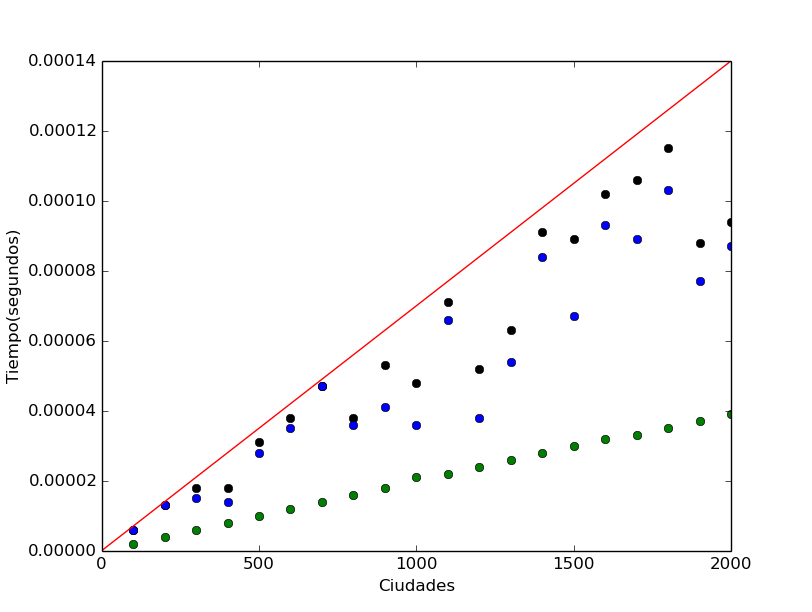
\includegraphics[width=450pt]{ej1_100a2000.png}
\caption{n=100 a 2000}
\end{figure}

Se tomó la función $f_1(n)=0.000007*n$.

Al parecer, la $f_1$ propuesta puede acotar fácilmente los valores tomados durante las mediciones de tiempo, y es una función lineal, por lo que los tests parecerían corroborar lo que asumimos.

En este caso se midieron los tiempos para $n$ entre 10000 y 200000, tomando los $n$ con 10000 ciudades de diferencia entre cada uno.

\begin{figure}[H]
\centering
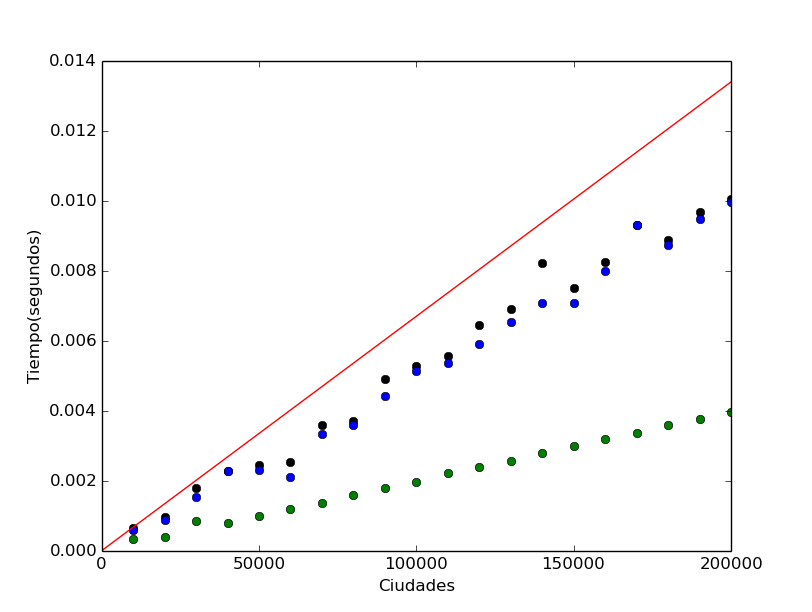
\includegraphics[width=450pt]{ej1_10000a200000.png}
\caption{n=100000 a 200000}
\end{figure}

Tomando la función $f_2(n)=0.00065*n$

Nuevamente, la $f_2$ propuesta demuestra ser capaz de acotar superiormente a los valores obtenidos como resultado de tomar mediciones de tiempo de la ejecución de nuestro programa, esta vez con un n 100 veces más grande.

Se puede notar una clara relación entre los tiempos obtenidos para las figuras 11 y 12.

Los puntos de referencia parecen haber requerido sólo variar sus valores en dos ceros, es decir tomando puntos 100 veces más grandes, por otro lado, $f_2$ es bastante parecido a 100 * $f_1$, y podría ser acotado fácilmente con 100 * $f_1$.

Estas observaciones parecen apoyar aún más la hipótesis de que la complejidad temporal es lineal.

\subsubsection{Terminación}

El algoritmo realiza llamadas a funciones auxiliares que no tienen ciclos, exceptuando a la función que crea las distancias entre las ciudad que tiene uno que itera sobre la cantidad de ciudades. 

Por otro lado, el ciclo principal del algoritmo también itera sobre la cantidad de ciudades y en cada iteración avanza una hasta llegar a la última, momento en el cual termina en ciclo.

\subsubsection{Correctitud}

Lo demostraremos por inducción en $n$ (siendo $n$ la cantidad de ciudades de un ramal). \\

\textbf{Caso base.} \\

Sólo hay una ciudad ($n$ = CantidadCiudades = 1, la capital), además, como inicializo los acumuladores de ciudades y de cable en cero: 

\begin{lstlisting}
  acumuladorDeCable1=0 acumuladorDeCiudades1=0
  acumuladorDeCable2=0 acumuladorDeCiudades2=0          
\end{lstlisting}

y por la inicialización de variables resulta que nunca entra en el ciclo principal

\begin{lstlisting}
  posCiudadInicial=CantidadCiudades - 2
  mientras posCiudadInicial >= 0 
\end{lstlisting}

Pero para $n$ = 1, \textsl{posCiudadInicial} = -1, por lo tanto el algoritmo retorna el máximo acumulado hasta el momento, igual a \textbf{0}. \\

\textbf{Paso Inductivo.} \\

Supongo que el algoritmo retorna la mayor cantidad posible de conexiones para \textbf{n-1} ciudades para un kilometraje \textsl{k}, quiero ver que retorna la mayor cantidad posible para \textbf{n} (es decir, si agrego una ciudad más al ramal) para dicha cantidad de kilómetros.

\textbf{Hay dos posibilidades:} o la ciudad \textbf{n} se encuentra a una distancia mayor de la cantidad de cable restante, o bien hay cable suficiente como para conectarla. \\

Si \textbf{alcanza el cable para conectar la ciudad} actualiza el acumulador de ciudades (sumando uno a la cantidad anterior)

\begin{lstlisting}
  si alcanzaElCable
    acumuladorDeCableActual = acumuladorDeCableActual + kmHastaEnesimaCiudad
    acumuladorDeCiudadesActual = acumuladorDeCiudadesActual++
\end{lstlisting}

y luego devuelve el máximo de los valores acumulados, con lo cual el valor de retorno es la mayor cantidad de ciudades que puedo conectar. \\

Si \textbf{no alcanza el cable para conectar la ciudad}, entonces la mayor cantidad posible de ciudades se logra en las primeras \textbf{n-1} ciudades, dado que, como mínimo, para agregar la ciudad \textbf{n} tengo que soltar una ciudad, y como sólo tengo sin analizar la ciudad \textbf{n} lo máximo que se va a conseguir es una ciudad más, razón por la cual era lo mismo quedarse con la resolución anterior.

\subsubsection{Ejemplos de casos borde}

\textbf{Varios intervalos de distintas cantidades de ciudades conectables:} \\

Como se ve en la figura Ejemplo1, el ramal tiene un intervalo al principio de 3 ciudades conectables, (del km 0 al 2) y luego tiene otro, (del km 20 al 23) que maximiza las conexiones, llevando la cantidad máxima a 4. El algoritmo analiza las primeras tres, y guarda en un acumulador 3, (ciudades conectables por el largo de cable dado). Luego, como no alcanza para conectar la ciudad de km 10, empieza a soltar ciudades, hasta que llega a la del km 20 y empieza a acumular hasta el km 23, que es lo máximo posible con el kilometraje de cable.

\begin{figure}[h]
\centering
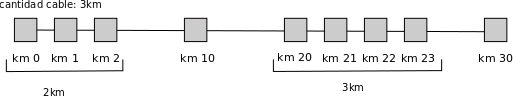
\includegraphics[scale = 0.7]{caso1}
\caption{Ejemplo1}
\label{Ejemplo1}
\end{figure}

\textbf{Soltar una ciudad para seguir analizando el ramal:} \\

En la figura Ejemplo2, la mayor cantidad de ciudades un momento antes de analizar el km 9 está entre el km 1 y el km8, luego, el algoritmo suelta la del km 1 para conectar el km 9 y ahí comienza a avanzar, conectando hasta el km 13, momento en el cual se acaba el kilometraje de cable dado. Como lo último que analiza es la conexión con el km 23, y no es conectable (no alcanza el cable), el valor de retorno del algoritmo de 8.

\begin{figure}[h]
\centering
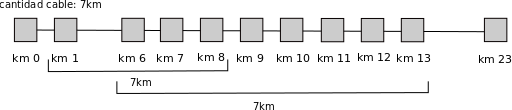
\includegraphics[scale = 0.7]{caso2}
\caption{Ejemplo2}
\label{Ejemplo2}
\end{figure}

\textbf{Soltar más de una ciudad para seguir analizando el ramal:} \\

En este caso, el algoritmo acumula desde la ciudad del km 1 al 7, luego debe soltar dos ciudades para realizar la conexión entre el km 7 y 13, y, por último, encuentra la mayor cantidad de ciudades conectables desde el km 13 al 18. Notar que no utiliza todo el largo de cable dado. (Ver figura Ejemplo3) 

\begin{figure}[h]
\centering
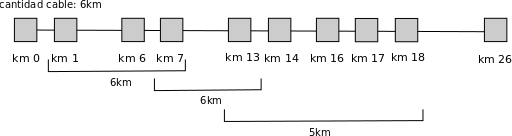
\includegraphics[scale = 0.7]{caso3}
\caption{Ejemplo3}
\label{Ejemplo3}
\end{figure}

\newpage
\textbf{La cantidad de cable dada no alcanza para conectar ningún par de ciudades:} \\

Como se ve en la figura Ejemplo4, sólo hay dos ciudades, la que está en el km 0 y la del km 10, pero la cantidad de kilómetros de cable no alcanza para conectarlas. En este caso, el algoritmo devuelve los acumuladores iniciales, que son seteados en 0, con lo cual obtenemos el valor esperado, que son 0 ciudades conectables.

\begin{figure}[h]
\centering
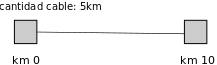
\includegraphics[scale = 0.7]{caso4}
\caption{Ejemplo4}
\label{Ejemplo4}
\end{figure}





Los ejemplos dados anteriormente cubren los distintos casos posibles del problema debido a que consideramos que el problema puede ser visto, mayormente, desde dos perspectivas distintas:

\begin{itemize}

\item Primero, nuestro algoritmo debe ser capaz de seleccionar, dentro de un subintervalo en el que hay varios casos óptimos, cuál es aquel que es más grande (y viable).

Esto queda demostrado en las últimas figuras, en los que se analizan los distintos comportamientos en las que puede caer nuestro algoritmo, y cómo estos son los adecuados para el problema planteado.

\item Segundo, se puede ver el problema como varios intervalos óptimos (algunos mejores que otros) separados por intervalos no-óptimos, este caso es analizado en la Figura 11.

Como el algoritmo recurre a guardar los mejores intervalos armados hasta el momento de uno de los dos acumuladores, cada vez que se arma uno de estos intervalos óptimos, se compara dicho intervalo con aquél guardado anteriormente, y se guarda aquel que sea mejor.

\end{itemize}

Así, ambas perspectivas han sido cubiertas y se comprueban los ejemplos de casos de dichos puntos de vista.


\newpage




%%%%%%%%%%%%%%%%%%%%%%%%%%%%%%%%%%%%%%%%%%%%%%%%%%%%%%%%%%%%%%%%%%%%%%%%%%%%%%%%%%%%%%%%%%%%%%%%%%%%%%%%%%
%%%%%%%%%%%%%%%%%%%%%%%%%%%%%%%%%%%%%%%%%%%%%%%%%%%%%%%%%%%%%%%%%%%%%%%%%%%%%%%%%%%%%%%%%%%%%%%%%%%%%%%%%%





\newcommand*{\boxednumber}[1]{%
    \expandafter\readdigit\the\numexpr#1\relax\relax
}
\newcommand*{\readdigit}[1]{%
    \ifx\relax#1\else
        \boxeddigit{#1}%
        \expandafter\readdigit
    \fi
}
% Format macro used for every digit, adjust to your liking:
\newcommand*{\boxeddigit}[1]{\fbox{#1}\hspace{-\fboxrule}}



\section{A Medias}


\subsection{El Problema}
\subsubsection{Introducción}
El problema a resolver requiere, dado un conjunto ordenado, es decir, una secuencia de enteros, encontrar una secuencia que en cada posición i contenga la mediana de la secuencia de entrada, con la mediana definida como:\\


$
mediana_{\ n \in \mathbb{N}\ |\ n = |\alpha|}(\alpha)=\begin{cases}
x_{\frac{n+1}{2}}& \text{si n es impar},\\
\frac{x_{\frac{n}{2}} + x_{\frac{n}{2} + 1}}{2}& \text{si n es impar}.
\end{cases}
$\\

\hfill

Es decir, para cada subsecuencia de la original entre 0 e i, el arreglo solución debe tener en la posición i la mediana de dicha subsecuencia.

\subsubsection{Ejemplo}

Dado el siguiente input,\\

\boxednumber{839154}\\


para el subarreglo de tamaño 1:\boxednumber{8}\\
el subarreglo ordenado es \boxednumber{8}\\
y el arreglo resultante devuelve su mediana en la posición 1:\boxednumber{8}\\

para el subarreglo de tamaño 2:\boxednumber{83}\\
el subarreglo ordenado es \boxednumber{38}\\
y el arreglo resultante devuelve su mediana en la posición 2:\boxednumber{85}\\

para el subarreglo de tamaño 3:\boxednumber{839}\\
el subarreglo ordenado es \boxednumber{389}\\
y el arreglo resultante devuelve su mediana en la posición 3:\boxednumber{858}\\

para el subarreglo de tamaño 4:\boxednumber{8391}\\
el subarreglo ordenado es \boxednumber{1389}\\
y el arreglo resultante devuelve su mediana en la posición 4:\boxednumber{8585}\\

para el subarreglo de tamaño 5:\boxednumber{83915}\\
el subarreglo ordenado es \boxednumber{13589}\\
y el arreglo resultante devuelve su mediana en la posición 5:\boxednumber{85855}\\

Finalmente, para el arreglo de tamaño 6:\boxednumber{839154}\\
el subarreglo ordenado es \boxednumber{134589}\\
y el arreglo resultante devuelve su mediana en la posición 6:\boxednumber{858554}\\
Este último arreglo es la solución del problema.

\subsection{El Algoritmo}

\subsubsection{Resumen}
El algoritmo lee los elementos de la secuencia de a uno, y los va almacenando en un $MinHeap$ y en un $MaxHeap$, de manera que en todo momento se cumpla que:
\begin{itemize}
\item Todos los elementos del $MinHeap$ son mayores a los del $MaxHeap$.
\item La diferencia entre la cantidad de elementos de los $heaps$ es a lo sumo 1.
\end{itemize}

De esta manera, para cada subsecuencia, los elementos quedan separados en dos mitades ($\pm 1$ un elemento).\\

Si la cantidad de elementos es par, la mediana viene dada por el promedio de las raíces de los $heaps$

Si la cantidad de elementos es impar, la mediana viene dada por la raiz del $heap$ con más elementos.

\subsubsection{Correctitud}

Veamos que el resultado es el esperado. En la sección anterior mencionamos que el algoritmo separa los elementos leídos hasta el momento en dos mitades($\pm 1$ un elemento).
\indent Además, para cada subsecuencia, si la cantidad de elementos es par, entonces ambos $heaps$ tienen la misma cantidad de elementos. Notar que las raíces de los $heaps$ se encuentran los elementos que están ubicados en la mitad del subarreglo de input ordenado, ya que son el mayor de la mitad menor, y el menor de la mitad mayor. En este caso, la mediana viene dada por el promedio entre las raíces.\\
\indent Si la cantidad de elementos es impar, entonces hay un $heap$ con un elemento más que el otro. En este caso, la raiz de dicho $heap$ es la mediana del subarreglo, ya que ese es el elemento que está ubicado en la mitad del arreglo.\\

Como el algoritmo hace esto último para cada subsecuencia y lo va guardando en un arreglo resultado, este arreglo resultado al terminar contiene las medianas de todos los subarreglos, que es lo que pedía el problema.

\subsubsection{Terminación}

Para ver que el algoritmo termina luego de una cantidad finita de estados, basta mostrar que el ciclo principal de la función $mediana$ termina. Dicho ciclo recorre los elementos en el arreglo S hasta llegar al último. El arreglo no se modifica ni se redimensiona en ningún momento, luego el ciclo termina.

Asumimos que todas las llamadas a procedimientos de la librería del lenguaje C++ terminan, si se cumple su precondición. Esto último es cierto para todas las llamadas que realizamos, por lo que dichas funciones terminan.



\subsubsection{Ejemplo}
Tomando el ejemplo de la sección 2.1.2, veremos que el algoritmo termina y da la solución correcta. Tenemos el siguiente input:\\

\boxednumber{839154}\\

El algoritmo crea un $MaxHeap$, que llamaremos $menores$ y un $MinHeap$, que llamaremos $mayores$ vacíos y comienza a recorrer el arreglo.\\
Primer iteración:\\
Toma el \boxednumber{8}, y como $menores$ está vacío lo inserta. Ahora $menores$ queda de la siguiente manera:\\

\begin{tikzpicture}[very thick,level/.style={sibling distance=70mm/#1}]
\node [vertex] (r){$8$}
  ;
\end{tikzpicture}\\
y $mayores$ está vacío.\\

Como $menores$ tiene más elementos, la mediana está en su raíz. El subarreglo solución queda:\\

\boxednumber{8}\\

Segunda iteración:\\
Toma el \boxednumber{3}, y lo compara con la raíz de $menores$. Como 3 \textless\ 8 debe insertarlo en $menores$, pero como el tamaño de $menores$ es mayor al de $mayores$, primero debe sacar la raiz y agregarla a $mayores$, para mantener los árboles con el mismo tamaño. Ahora $menores$ queda de la siguiente manera:\\

\begin{tikzpicture}[very thick,level/.style={sibling distance=70mm/#1}]
\node [vertex] (r){$3$}
  ;
\end{tikzpicture}\\
y mayores queda de la siguiente manera:\\

\begin{tikzpicture}[very thick,level/.style={sibling distance=70mm/#1}]
\node [vertex] (r){$8$}
  ;
\end{tikzpicture}\\

Como $menores$ y $mayores$ tienen la misma cantidad de elementos, la mediana viene dada por la parte entera del promedio de las raíces de ambos, que se agrega al subarreglo solución:\\

\boxednumber{85}\\

Tercer iteración:\\
Toma el \boxednumber{9}, y lo compara con la raíz de $menores$. Como 9 \textgreater\ 3, lo inserta en $mayores$.

$menores$:\\

\begin{tikzpicture}[very thick,level/.style={sibling distance=70mm/#1}]
\node [vertex] (r){$3$}
  ;
\end{tikzpicture}

$mayores$:\\

\begin{tikzpicture}[very thick,level/.style={sibling distance=70mm/#1}]
\node [vertex] (r){$8$}
  child {
    node [vertex] (a) {$9$}
  }
;
\end{tikzpicture}

Como $mayores$ tiene más elementos, la mediana está en su raíz. Ésta se agrega al subarreglo solución:\\

\boxednumber{858}\\

Cuarta iteración:\\
Toma el \boxednumber{1}, y lo compara con la raíz de $menores$. Como 1 \textless\ 3, lo inserta en $menores$. $menores$ y $mayores$ quedan:

\begin{tikzpicture}[very thick,level/.style={sibling distance=70mm/#1}]
\node [vertex] (r){$3$}
  child {
    node [vertex] (a) {$1$}
  };
\end{tikzpicture} \hspace*{20pt}
\begin{tikzpicture}[very thick,level/.style={sibling distance=70mm/#1}]
\node [vertex] (r){$8$}
  child {
    node [vertex] (a) {$9$}
  }
;
\end{tikzpicture}

Como $menores$ y $mayores$ tienen la misma cantidad de elementos, la mediana viene dada por la parte entera del promedio de las raíces de ambos, que se agrega al subarreglo solución:\\

\boxednumber{8585}\\

Quinta iteración:\\
Toma el \boxednumber{5}, y lo compara con la raíz de $menores$. Como 5 \textgreater\ 3, debe insertarlo en $mayores$. $menores$ y $mayores$ quedan:

\begin{tikzpicture}[very thick,level/.style={sibling distance=70mm/#1}]
\node [vertex] (r){$3$}
  child {
    node [vertex] (a) {$1$}
  };
\end{tikzpicture} \hspace*{20pt}
\begin{tikzpicture}[very thick,level/.style={sibling distance=30mm/#1}]
\node [vertex] (r){$5$}
  child {
    node [vertex] (a) {$8$}
  }
  child {
    node [vertex] (a) {$9$}
  }
;
\end{tikzpicture}


Como $mayores$ tiene más elementos, la mediana está en su raiz. Esta se agrega al subarreglo solución:\\

\boxednumber{85855}\\

Sexta iteración:\\
Toma el \boxednumber{4}, y lo compara con la raiz de $menores$. Como 4 \textgreater   3, debe insertarlo en $mayores$. Primero saca la raiz de $mayores$ y la inserta en $menores$. $menores$ y $mayores$ quedan:\\

\begin{tikzpicture}[very thick,level/.style={sibling distance=30mm/#1}]
\node [vertex] (r){$5$}
  child {
    node [vertex] (a) {$3$}
  }
  child {
    node [vertex] (a) {$1$}
  };
\end{tikzpicture} \hspace*{20pt}
\begin{tikzpicture}[very thick,level/.style={sibling distance=30mm/#1}]
\node [vertex] (r){$4$}
  child {
    node [vertex] (a) {$8$}
  }
  child {
    node [vertex] (a) {$9$}
  }
;
\end{tikzpicture}

Como $menores$ y $mayores$ tienen la misma cantidad de elementos, la mediana viene dada por la parte entera del promedio de las raíces de ambos, que se agrega al arreglo solución:\\

\boxednumber{858554} \hspace*{3pt} que es la solución del problema. \\

\subsection{Complejidad temporal}
El algoritmo resuelve el problema en $\mathcal{O}(n \log n)$ y $\Omega(n)$. La función $mediana$ recorre el arreglo, y para cada elemento hace una llamada a la función $medianaSubarreglo$.

\begin{algorithm}
\caption{\ \ \ \ \ \ \ \ \textbf{void} mediana(\textbf{arreglo} \textit{S}) \ \ \ \ \ \ \ \ \ \ \ \ \ \ \ \ \ \ \ \ \ \ \ \ \ \ \ \ \ $\mathcal{O}(n\log{}n)$}
\label{alg2}        % label for \ref{} commands later in the document
\begin{algorithmic}

    \FOR{cada elemento en S}
        \STATE Llamar a medianaSubarreglo para el elemento actual \ \ \ \ \ \ \ \ \ \ \ \ \ \ \ \ \ \ \ \ $\mathcal{O}(\log_2 n)$
        \STATE Guardar el resultado de medianaSubarreglo en la posición actual \ \ \ \ $\mathcal{O}(1)$
    \ENDFOR

\end{algorithmic}
\end{algorithm}


\begin{algorithm}
\caption{\ \ \ \ \textbf{int} medianaSubarreglo(\textbf{int} elem, \textbf{heap} mayores, \textbf{heap} menores)  \ \ \ \ \ \ \ \ \ \ \ \ \ \ $\mathcal{O}(\log{}n)$}
\label{alg2}        % label for \ref{} commands later in the document
\begin{algorithmic}

    \IF{\textit{menores} está vacia}
        
        \STATE Agregar \textit{elem} a \textit{menores}
        
    \ELSE
        \IF{\textit{elem} $<$ raíz de \textit{menores}}
        
            \IF{tamaño de \textit{menores} $>$ tamaño de \textit{mayores}}
                \STATE Agregar a \textit{mayores} la raíz de \textit{menores}
                \STATE Sacar la raíz de \textit{menores}
                \STATE Agregar \textit{elem} a \textit{menores}
            \ELSE
                \STATE Agregar \textit{elem} a \textit{menores}
            \ENDIF
            
        \ELSE
        
            \IF{tamaño de \textit{mayores} $>$ tamaño de \textit{menores}}
            
                \STATE Agregar a \textit{menores} la raíz de \textit{mayores}
                \STATE Sacar la raíz de \textit{mayores}
                \STATE Agregar \textit{elem} a \textit{mayores}
        
            \ELSE
        
                \STATE Agregar \textit{elem} a \textit{mayores}
            
            \ENDIF
        \ENDIF
    \ENDIF
    
    \RETURN raíz del \textit{heap} con más elementos (o el promedio de las raices si tienen la misma cantidad)

\end{algorithmic}
\end{algorithm}


Para esta implementación puntual, utilizamos el $heap$ provisto por el lenguaje (C++) con un $vector$ como $underlying$ $container$. Este garantiza las operaciones de empty(), size() y top() en tiempo constante.

El tiempo de la operación de push() es la suma de los tiempos de la operación push\textunderscore back() de $vector$ más la operación push\textunderscore heap(). Push\textunderscore back() toma tiempo constante amortizado, ya que puede ser necesario reubicar el vector. Como el costo de hacer $n$ operaciones de push\textunderscore back() sobre el vector a lo largo de todo el algoritmo es $\mathcal{O}(n)$, y a lo sumo se realizan n/2 push() en cada heap, podemos asegurar que todos los push\textunderscore back() se realizan en tiempo constante. Push\textunderscore heap() garantiza tiempo logarítmico en el tamaño del heap. Luego push() se realiza en tiempo logarítmico.

El tiempo de la operación de pop() es la suma de los tiempos de la operación pop\textunderscore heap() más la operación pop\textunderscore back de $vector$. El lenguaje garantiza pop\textunderscore heap() en tiempo dos veces logaritmico en el tamaño del heap, y pop\textunderscore back() en tiempo constante. Luego pop() se realiza en tiempo logarítmico.




\subsubsection{Peor caso}

La función \textit{medianaSubarreglo} recibe como parámetro los dos \textit{heaps} y el elemento actual, y lo inserta en el \textit{heap} correspondiente. Para saber dónde insertar, obtiene la raíz de \textit{menores} en $\mathcal{O}(1)$ y la compara con el elemento. Para el caso en que el \textit{heap} en el que se va a insertar el elemento tiene un elemento más que el otro \textit{heap}, primero hay que sacar la raíz del que más elementos tiene para mantenerlos con igual tamaño. Este es el caso en que más operaciones realiza: \textbf{(1)} Obtiene la raíz del \textit{heap} que más elementos tiene en $\mathcal{O}(1)$, \textbf{(2)} La agrega al otro \textit{heap} en $\mathcal{O}(\log_2 n)$, \textbf{(3)} Elimina dicha raíz en $\mathcal{O}(\log_2 n)$, y \textbf{(4)} Agrega el elemento al \textit{heap} en el que hizo lugar en $\mathcal{O}(\log_2 n)$. Es decir, en el peor de los casos realiza $\mathcal{O}(3 \log_2 n)$ más una cantidad acotada de comparaciones.



\subsubsection{Mejor caso}
Hay un mejor caso, en el que el arreglo A de input cumple que:

\begin{itemize}
\item Hay un subarreglo B del arreglo original, que no tiene más de dos elementos consecutivos en el arreglo original y que cumple el invariante de MaxHeap.
\item Hay un subarreglo C del arreglo original, que no tiene más de dos elementos consecutivos en el arreglo original y que cumple el invariante de MinHeap.
\item Los subarreglos mencionados son disjuntos.
\item Para todo \textit{i} entre 0 y el tamaño del arreglo -1, el subarreglo consecutivo A[0..i] tiene la misma cantidad de elementos en B y en C ($\pm$1 elemento).
\end{itemize}

En este caso, todas las inserciones en los \textit{heaps} son en $\mathcal{O}(1)$, ya que todos los elementos se insertan al final de cada \textit{heap} y no hace falta rebalancearlos, ni sacar elementos. En este caso, las medianas de todos los subarreglos siempre son alguno de los dos primeros elementos del arreglo original (o el promedio entre ambos). Para un input de esta forma, el algoritmo realiza \textit{n} llamadas a $medianaSubarreglo$, que realiza una cantidad constante de operaciones elementales, por lo que $mediana$ está en $\Omega(n)$.

\boxednumber{564738291} es un ejemplo de mejor caso, donde

\boxednumber{5} \ \ \ \boxednumber{4}\ \ \ \boxednumber{3}\ \ \ \ \boxednumber{2}\ \ \ \boxednumber{1} caen en un $heap$, y

\ \ \ \ \boxednumber{6} \ \ \ \boxednumber{7}\ \ \ \boxednumber{8}\ \ \ \ \boxednumber{9} caen en el otro.



\newpage




%%%%%%%%%%%%%%%%%%%%%%%%%%%%%%%%%%%%%%%%%%%%%%%%%%%%%%%%%%%%%%%%%%%%%%%%%%%%%
%%%%%%%%%%%%%%%%%%%%%%%%%%%%%%%%%%%%%%%%%%%%%%%%%%%%%%%%%%%%%%%%%%%%%%%%%%%%%

\section{Girls Scouts}

\subsection{El Problema}
 \subsubsection{Introducción}
Se plantea en este caso el problema de, dados:
\begin{itemize}

\item Un conjunto de niñas exploradoras.

\item Las relaciones de amistad entre ellas, es decir, para cada niña, sus amigas dentro del grupo de exploradoras.
\end{itemize}

Hallar la manera de sentarlas en una ronda, de manera tal que las niñas que son amigas, estén a una distancia mínima. Formalmente dicho, se pide que la sumatoria de las distancias entre todos los pares de amigas, sea la mínima. Como resultado, se debe devolver la distancia máxima entre los pares de amigas de la ronda, junto con la misma. 

El algoritmo debe funcionar con orden de complejidad estrictamente mejor que O($e^{e}  a^{2}$), donde \textbf{e} es la cantidad de exploradoras, y \textbf{a} es la cantidad de amistades.

\subsubsection{Ejemplos}

\vspace{2mm}
\textbf{Ejemplo 1}
\vspace{2mm}

A modo de ejemplo de qué plantea el problema, y sus soluciones, se observan casos:\\ 

Dado el grupo de exploradoras conformado por \{a, b, c, d, e\}, y sus respectivas amistades: 

\begin{center}
\{\{a,b\}\{a,c\}\{a,d\}\{a,e\}\{b,c\}\{b,d\}\{b,e\}\{c,d\}\{c,e\}\}
\end{center}

Notar que utilizamos un conjunto de conjuntos para ejemplificar las amistades porque estas son simétricas, lo que quiere
decir que si \textbf{a} es amiga de \textbf{b} entonces \textbf{b} es amiga de \textbf{a}. Cada una de las
amistades tiene su correspondiente distancia en la ronda. Por ejemplo, una posible manera de sentarlas es:

\begin{figure}[H]
\begin{center}
  \begin{tikzpicture}
    \hspace*{0.5cm}
    \node [fill=gray!30] (a) at (0,0) { a };
    \node [fill=gray!30] (b) at (2,2) { b };
    \node [fill=gray!30] (c) at (1,4) { c };
    \node [fill=gray!30] (d) at (-1,4) { d };
    \node [fill=gray!30] (e) at (-2,2) { e };
    
    \begin{pgfonlayer}{bg}    % select the background layer
      %%        \draw (0) (a)--(b) (22);
      %%        \draw (0) (e)--(b);
    \end{pgfonlayer}
  \end{tikzpicture}
\end{center}
\end{figure}

Donde la sumatoria de las distancias entre todos los pares de amigas en esta ronda es 14.
\begin{itemize}
  \item d(a,b) = 1   \ \ \ \inlineitem d(a,c) = 2 \ \ \ \inlineitem d(a,d) = 2
  \item d(a,e) = 1   \ \ \ \inlineitem d(b,c) = 1 \ \ \ \inlineitem d(b,d) = 2
  \item d(b,e) = 2   \ \ \ \inlineitem d(c,d) = 1 \ \ \ \inlineitem d(c,e) = 2
\end{itemize}

Donde d(x,y) es la distancia entre x e y.

Como el problema nos pedía la ronda cuya distancia entre los pares de amigas sea la mínima, podemos 
ver intuitivamente como esta ronda no es óptima ya que \textbf{d} y \textbf{e} no son amigas, sin embargo
están sentadas juntas (a distancia 1). Como en este caso la cantidad mínima de amistades que tiene
una exploradora es 3, no puede haber una solución óptima donde sentemos juntas a dos que no son amigas.
Podemos ver como al separarlas obtenemos una ronda mejor (cuya distancia total entre todos los
pares de amigas es menor):

\begin{figure}[H]
\begin{center}
  \begin{tikzpicture}
    \hspace*{0.5cm}
    \node [fill=gray!30] (a) at (0,0) { a };
    \node [fill=gray!30] (b) at (2,2) { b };
    \node [fill=gray!30] (c) at (1,4) { d };
    \node [fill=gray!30] (d) at (-1,4) { c };
    \node [fill=gray!30] (e) at (-2,2) { e };
    
    \begin{pgfonlayer}{bg}    % select the background layer
      %%        \draw (0) (a)--(b) (22);
      %%        \draw (0) (e)--(b);
    \end{pgfonlayer}
  \end{tikzpicture}
\end{center}
\end{figure}

\begin{itemize}
  \item d(a,b) = 1   \ \ \ \inlineitem d(a,c) = 2 \ \ \ \inlineitem d(a,d) = 2
  \item d(a,e) = 1   \ \ \ \inlineitem d(b,c) = 2 \ \ \ \inlineitem d(b,d) = 1
  \item d(b,e) = 2   \ \ \ \inlineitem d(c,d) = 1 \ \ \ \inlineitem d(c,e) = 1
\end{itemize}

Por ende, la sumatoria de las distancias entre todos los pares de amigas en esta ronda es 13.
\vspace{2mm}
\textbf{Ejemplo 2}\\
\vspace{2mm}
Dado el grupo de exploradoras conformado por \{a, b, c\} donde ninguna es amiga de otra. En este caso tenemos que 
cualquier manera de sentar al grupo de exploradoras es solución al problema, porque no hay ninguna restricción al respecto.

Como todas las posibles permutaciones de la ronda son soluciones posibles, al ser \{a, b, c\} la menor lexicográficamente, 
es la solución al problema.

\subsection{Estructuras}

En esta sección discutiremos las posibles estructuras de representación que podrían ser utilizadas
para la resolución de este problema, y justificaremos nuestra elección.

Para el conjunto de exploradoras, lo importante es que queremos modelar una ronda. Sin importar
qué utilicemos efectivamente para representarla, consideramos de suma importancia (por el uso de abstracción,
declaratividad, y modularización del problema) utilizar una clase hecha por nosotros que modele el 
comportamiento de la ronda.

Posibles estructuras que se pueden utilizar para implementar las rondas son: 
\begin{itemize}
\item Lista simple o doblemente enlazada
\item Lista circular
\item Arreglo
\item Vector
\end{itemize}
La estructura que utilizamos para resolver el problema de representación de la Ronda 
fue un Vector que modela el comportamiento de una 
lista circular a través de las operaciones provistas por la clase Ronda. Por ejemplo [a,b,c,d,e] es una 
posible representación de la ronda donde, teniendo en cuenta el hecho de que es circular,
se puede observar la distancia entre \textbf{a} y \textbf{e} es 1 en vez de 4 porque del último se puede llegar al primero.

Por el otro lado sus respectivas amistades se pueden representar, por ejemplo, con:
\begin{itemize}
\item Matriz de booleanos (1 indica amistad, 0 no).
\item Diccionario con claves exploradoras y significado sus amigas.
\item Lista de listas.
\item Conjunto de conjuntos.
\end{itemize}
La estructura que utilizamos para resolver el problema de representación de las amistades fue un conjunto de
conjuntos, ya que nos interesó representar la simetría entre las amistades y que, por ejemplo, la amistad 
\{a,b\} es igual a \{b,a\}.

Además, nuestro contexto de uso (del cual se desprende la complejidad) no 
nos impuso ninguna restricción que no permitiera el uso de alguna de las estructuras mencionadas previamente.

\subsection{El Algoritmo}

\subsubsection{Complejidad}

En esta sección mostraremos un pseudocódigo de nuestra implementación, junto con su explicación y justificación
de complejidad.

La idea del algoritmo utilizado para resolver el problema fue, dado que tenemos que encontrar la ronda 
que mínimiza la sumatoria de la distancias, generar todas las posibles permutaciones de la ronda de exploradoras
y elegir la óptima. Para comparar entre dos rondas cuál es mejor a la solución del problema, 
recorremos el conjunto de amistades y para cada una de ellas sumamos su distancia en un acumulador. Luego, nos quedamos
con aquella para la que dicha sumatoria sea menor.

Sólo por un tema de notación, al conjunto de conjuntos de char lo renombramos como bigSet, para hacer menos 
engorroso el código.
\\ \\
\noindent\makebox[\linewidth]{\rule{17cm}{0.4pt}}
\algoritmo{rondaOptima}{in/out rondaRes : Tupla(Ronda\, int),in/out exploradoras : Ronda,in amistades : bigSet}{res : string}{
  \Var{n : int}
  \complejidad{O(1)}
  \State $n \larr exploradoras.cantidad()$
  \complejidad{O(1)}
  \If{(amistades.size() $\neq$ 0 $\wedge$ amistades.size() $\neq$ $\frac{n*(n-1)}{2}$)}
  \complejidad{O(1)}
  \State $permutaciones(rondaRes, exploradoras, 0, amistades)$
  \complejidad{O($e!*e*a$)}
  \Else
  \State $\Pi_0{(rondaRes)}.ordenar()$
  \complejidad{O($e^2$)}
  \EndIf
  \Var{dist: int}
  \complejidad{O(1)}
  \State $dist\larr \Pi_0{(rondaRes)}.maxDistAmistades(amistades)$
  \complejidad{O($e*a$)}
  \State $res.append(dist)$
  \complejidad{O(1)}
  \State $res.append(" ")$
  \complejidad{O(1)}
  \Var{i: int}
  \complejidad{O(1)}
  \For {i = 0 \textbf{to} $\Pi_0{(rondaRes)}.cantidad()$}
  \complejidad{O($e^{2}$)}
  \State $res.push\_back(\Pi_0{(rondaRes)}.exploradoraEnPos(i))$
  \complejidad{O($e$)}
  \EndFor
} {O($e!*e*a + e*a + e^2$)}

\vspace{1mm}
Nota: $\Pi_0$ y $\Pi_1$ son utilizados para referirse al primer y segundo elemento de las tuplas.

\vspace{3mm}
\begin{center}
\textbf{Explicación y justificación de complejidad} \\ 
\end{center} 

La complejidad del algoritmo es O($e!*e*a + e*a + e^{2}$).

Observamos primero la suma entre ($e!*e*a + e^{2}$)
\begin{itemize}
\item Como $e! = (e*(e-1)*(e-2)*...*1) > e \\ \implies $ $e \in$ O($e!$). \\ Luego, podemos escribir a 
  ($e!*e*a + e^2$) = ($e *(e!*a + e)$) $\in$ O($e *(e!*a + e)$) \\ $\implies$ O($e*max(e!*a, e)$) \\ lo cual, por lo demostrado anteriormente, es equivalente a O($e!*a*e$)
\item Como ($e!*e*a + e*a$) = ($e*a (e! + 1)$) $\in$ O($(e!*e*a)$)
\end{itemize}
Luego, la complejidad total del algoritmo es O($e!*e*a)$).

Nuestro algoritmo cumple con la cota de complejidad provista por la cátedra ya que:
\begin{itemize}
  \item Como $e! = (e*(e-1)*(e-2)*...*3*2*1) < e^{e-1}$ \\ $\implies$ $e! < e^{e-1}$ \\ $\implies$ $e!*e < e^{e-1}*e 
    = e^{e}$ \\ $\implies$ $e! \in$ O($e^e$) \\
    Luego, como $e! < e^e$ y $a$ $\in$ \mathbb{N}\\ $\implies$ $e!*a < e^e*a < e^e*a^2$
\end{itemize}
Por lo cual, demostramos que la complejidad del algoritmo es O($e!*e*a$) $\in$ O($e^e*a^2$).
Como la complejidad de las funciones \textbf{permutaciones} 
y \textbf{maxDistAmistades} las justificaremos con su debido código, en esta parte explicaremos el resto del 
algoritmo. 

Utilizamos las operaciones \textbf{append} y \textbf{push\_back} que cumplen la misma función en cuanto a que
concatenan al final del string el string o caracter pasado por parámetro, pero por problema de tipos, 
utilizamos las dos en los distintos casos. Ambas operaciones son lineales en la cantidad de elementos del nuevo string concatenado.
Las primeras dos concatenaciones mediante la función \textbf{append} al resultado cuestan O(1) ya que, al 
tener solo dos elementos, esas operaciones son de costo constante.

Luego, el ciclo \textbf{for} que itera sobre el conjunto de exploradoras resultante cicla $e$ veces. En cada
iteración se llama a la función \textbf{push\_back} que le concatena al string el nuevo caracter pasado por parámetro.
En total el ciclo cuesta:

\begin{center}
$\sum\limits_{i=2}^e i = \frac{e*(e-1)}{2} - 1 \in O(e^2)$
\end{center}

Por último, las complejidades de \textbf{exploradoraEnPos} y \textbf{cantidad} son constantes ya que están
directamente implementadas con el operator $[]$ y la función $size()$ de la clase Vector de c++.

Ahora pasaremos a demostrar las complejidades de los algoritmos auxiliares.
\\ \\
\noindent\makebox[\linewidth]{\rule{17cm}{0.4pt}}
\algoritmo{permutaciones}{in/out rondaRes : Tupla(Ronda int),in/out exploradoras : Ronda,in pos : int,in amistades : bigSet}{}{
\If{(pos == exploradoras.cantidad())}
\complejidad{O(1)}
\Var{sumaDists : int}
\complejidad{O(1)}
\State $sumaDists \larr exploradoras.sumaDistancias(amistades)$
\complejidad{O($e*a$)}
\If{(sumaDists $< \Pi_0(rondaRes)$)}
\complejidad{O(1)}
\State $\Pi_0(rondaRes) \larr exploradoras$
\complejidad{O($e$)}
\State $\Pi_1(rondaRes) \larr sumaDists$
\complejidad{O(1)}
\EndIf
\If{((sumaDists == $\Pi_0(rondaRes)) \wedge (exploradoras < \Pi_0(rondaRes)$))}
\complejidad{O($e$)}
\State $\Pi_0(rondaRes) \larr exploradoras$
\complejidad{O($e$)}
\EndIf
\Else
\Var{i : int}
\complejidad{O(1)}
\For{(i = 0 \textbf{to} exploradoras.cantidad())}
\State $exploradoras.swap(pos, i)$
\complejidad{O(1)}
%  \If{exploradoras.exploradoraEnPos(pos, i)}
\State $permutaciones(rondaRes, exploradoras, pos+1, amistades)$
\complejidad{O(1)}
\State $exploradoras.swap(pos, i)$
\complejidad{O(1)}
\EndFor
\EndIf
} {O($e*a$)}

\vspace{3mm}
\begin{center}
\textbf{Explicación y justificación de complejidad} \\ 
\end{center} 

La idea del algoritmo es ir generando todas las permutaciones posibles del conjunto de exploradoras y, en el 
caso base, quedarse con la secuencia de exploradoras cuya sumatoria de distancias entre 
amigas es menor. En caso de que sean iguales, se considera como menor a la menor lexicográficamente. 

Para analizar la complejidad del algoritmo es necesario ver cuántas llamadas recursivas realiza.
\begin{itemize}
\item Cuando pos = 0 (su valor inicial), el algoritmo realiza $e$ llamadas recursivas.
\item Cuando pos = 1 el algoritmo realiza $e-1$ llamadas recursivas.
\item Cuando pos = n el algoritmo realiza $e-n$ llamadas recursivas.
\end{itemize}

Lo cual, al generalizar nos queda la recurrencia de la manera:

\vspace{1mm}

\[ T(e) = 
  \begin{cases} 
    e * T(e-1) & \mbox{si} \ e \ \neq \mbox{1} \\
    1 & \mbox{si} \ e \ \mbox{= 1} 
  \end{cases}
\]

\vspace{2mm}

Entonces, como hago $e!$  llamadas a una función que tiene orden de complejidada O($e*a$) la complejidad 
total es O($e!*e*a$).

\begin{center}
$T(e) = e * T(e-1) = \prod_{i=1}^{e} i = e! \in O(e!)$
\end{center}

\vspace{5mm}
\noindent\makebox[\linewidth]{\rule{17cm}{0.4pt}}

.
\\
\algoritmo{sumaDistancias}{in/out exploradoras : Ronda,in amistades : bigSet}{res : int}{
\Var{exp1 : char}
\complejidad{O(1)}
\Var{exp2 : char}
\complejidad{O(1)}
\Var{acum : int}
\complejidad{O(1)}
\Var{itA : amistades.CrearIterador()}
\complejidad{O(1)}
\While{itA.siguiente() != NULL}
\complejidad{O($a$)}
\State $exp1 \larr primerElem(itA)$
\complejidad{O(1)}
\State $exp2 \larr segundoElem(itA)$
\complejidad{O(1)}
\State $acum \larr acum + distancia(exploradoras, exp1,exp2)$
\complejidad{O($e$)}
\EndWhile
\State $res \larr acum$
\complejidad{O(1)}
}{O($e*a$)}

\vspace{3mm}
\begin{center}
\textbf{Explicación y justificación de complejidad} \\ 
\end{center} 
La idea del algoritmo es ir recorriendo el conjunto de amistades y, por cada amistad, almacenar el valor de 
su distancia en la ronda en un acumulador.

El ciclo itera $a$ veces ya que cicla sobre todo el conjunto de amistades. Las operaciones que obtiene el 
primer y segundo elemento del conjunto amistad son O(1) ya que el tamaño de ese conjunto está acotado por 
2 (las amistades son de a pares). Luego obtiene la distancia entre las dos exploradoras llamando a la 
función \textbf{distancia} la cual es lineal en la cantidad de exploradoras. Por ende la complejidad
total del ciclo, y de la función, es de orden O($e*a$). \\
\noindent\makebox[\linewidth]{\rule{17cm}{0.4pt}}
.
\\
\algoritmo{distancia}{in exploradoras : Ronda,in exp1 : char,in exp2 : char}{res : int}{
\Var{posExp1 : char}
\complejidad{O(1)}
\Var{posExp2 : char}
\complejidad{O(1)}
\Var{dist1: int}
\complejidad{O(1)}
\Var{dist2: int}
\complejidad{O(1)}
\State $posExp1 \larr encontrarPos(exp1)$
\complejidad{O($e$)}
\State $posExp2 \larr encontrarPos(exp2)$
\complejidad{O($e$)}
\State $dist1 \larr abs(posExp1 - posExp2)$
\complejidad{O(1)}
\State $dist2 \larr exploras.size() - dist1$
\complejidad{O(1)}
\State $res \larr min(dist1, dist2)$
\complejidad{O(1)}
}{O($e$)}

\begin{center}
\textbf{Explicación y justificación de complejidad} \\ 
\end{center} 

La idea del algoritmo es encontrar las posiciones de las exploradoras en la ronda y luego, como modelamos 
una lista circular, tener en cuenta que del primero se puede ir al último. Por eso se busca el mínimo entre
la distancia estándar en cualquier arreglo, y la distancia obtenida cuando se puede ir del primero al último.
Como buscar las posiciones dentro de la ronda de las exploradoras es lineal en la cantidad de exploradoras 
el algoritmo tiene orden de complejidad O($e$).

\noindent\makebox[\linewidth]{\rule{17cm}{0.4pt}}
.\\
\algoritmo{encontrarPos}{in exploradoras : Ronda,in exp : char}{res : int}{
\Var{i : int}
\complejidad{O(1)}
\State $i \larr 0$
\complejidad{O(1)}
\While{i $<$ exploradoras.size()}
\complejidad{O($e$)}
\If{exp == exploradoras[i]}
\complejidad{O(1)}
\State $res \larr i$
\complejidad{O(1)}
\EndIf
\State $i \larr i+1$
\complejidad{O(1)}
\EndWhile
} {O($e$)}

\vspace{3mm}
\begin{center}
\textbf{Explicación y justificación de complejidad} \\ 
\end{center} 

La idea del algoritmo es realizar una búsqueda secuencial en la ronda, la cual es lineal en la cantidad de 
exploradoras, y por ende, el algoritmo tiene orden de complejidad O($e$).

\noindent\makebox[\linewidth]{\rule{17cm}{0.4pt}}
.\\
\algoritmo{maxDistAmistades}{in/out exploradoras : Ronda,in amistades : bigSet}{res : int}{
\Var{exp1 : char}
\complejidad{O(1)}
\Var{exp2 : char}
\complejidad{O(1)}
\Var{acum : int}
\complejidad{O(1)}
\Var{itA : amistades.CrearIterador()}
\complejidad{O(1)}
\While{itA.siguiente() != NULL}
\complejidad{O($a$)}
\State $exp1 \larr primerElem(itA)$
\complejidad{O(1)}
\State $exp2 \larr segundoElem(itA)$
\complejidad{O(1)}
\State $acum \larr max(acum, distancia(exploradoras, exp1,exp2))$
\complejidad{O($e$)}
\EndWhile
\State $res \larr acum$
\complejidad{O(1)}
}{O($e*a$)}

\vspace{3mm}
\begin{center}
\textbf{Explicación y justificación de complejidad} \\ 
\end{center} 

La idea del algoritmo es ir recorriendo el conjunto de amistades y en cada iteración elegir la amistad que está   
a una distancia máxima en la ronda.

El ciclo itera $a$ veces ya que cicla sobre todo el conjunto de amistades. Las operaciones que obtienen el 
primer y segundo elemento del conjunto amistad son O(1) ya que el tamaño de ese conjunto está acotado por 
2 (las amistades son de a pares). Luego obtiene la distancia entre las dos exploradoras llamando a la 
función \textbf{distancia} la cual es lineal en la cantidad de exploradoras. Por ende la complejidad
total del ciclo, y de la función, es O($e*a$). 

\subsubsection{Correctitud}

En esta sección mostraremos que la solución obtenida por el algoritmo es la pedida por el problema. 

El problema pide encontrar la ronda cuya sumatoria de las distancias entre los pares de amigas sea la menor.
Nuesta solución al problema fue calcular todas las posibles permutaciones de la ronda de exploradoras, por lo cual 
exploramos todas las posibles soluciones a la manera de sentar las exploradoras. Para cada solución nos fijamos 
si es la que provee en ese momento de ejecución del algoritmo la menor sumatoria de distancias. Como nuestro 
algoritmo evalúa todo el conjunto de posibles soluciones del problema, y se queda en cada caso base con la mejor,
podemos asegurar que el algoritmo es una solución correcta al problema, que cumple con las postcondiciones.

Existen dos casos especiales en los cuales no es necesario calcular todas las permutaciones del conjunto de exploradoras.
\begin{itemize}
  \item Cuando la cantidad de amistades es nula, es decir, cuando ninguna exploradora es amiga de otra.
  \item Cuando todas las exploradoras son amigas de todas.
\end{itemize}
Para estos dos casos lo único que hay que hacer es ordenar lexicográficamente la ronda de menor a mayor. 
Resultan ser los mejores casos del algoritmo ya que cualquier manera de sentar a las exploradoras 
es una solución posible.

En el primer caso se puede notar que no hay ninguna restricción en cuanto a cómo sentarlas 
ya que no hay necesidad de sentar a ninguna al lado de la otra.

En el segundo caso, como todas las exploradoras 
son amigas entre sí no hay manera de diferir en el resultado. En cualquier permutación posible toda exploradora va a tener al lado suyo 
a dos de sus amigas y como máximo a distancia $\lfloor$ $\frac{e}{2}$ $\rfloor$ de una amiga si $e$ es par, o de 
dos amigas si $e$ es impar. 

Luego, el resultado provisto es la ronda de exploradoras ordenada lexicográficamente, la cual es la solución 
al problema en estos casos.

Podemos saber cuál es el tamaño máximo del conjunto de amistades ya que 
se podría pensar al peor caso de las amistades como un grafo completo, donde todos los vértices (exploradoras) estan
relacionados con todos los otros. Como sabemos que la cantidad total de aristas de un grafo G(V,X) es:

\vspace{3mm}

\begin{center}
$\sum\nolimits_{i \in V}d(i) = 2m$ 
\end{center}

\vspace{3mm}

Donde $V$ es la cantidad de vértices, $d(i)$ su grado, siendo el grado de un vértice la 
cantidad de aristas incidentes a ese él, y $m$ la cantidad de aristas total del grafo. Entonces, como
m sería la cantidad total de amistades y si toda exploradora tiene $e-1$ amigas tenemos que:

\vspace{3mm}

\begin{center}
$m = \frac{\sum\limits_{i=1}^e (e-1)}{2} = \frac{e*(e-1)}{2}$
\end{center}

\vspace{3mm}

Con lo cual sabemos que cuando el conjunto de amistades tiene longitud cero o $m$ podemos afirmar que estamos 
en uno de estos dos casos.





\subsubsection{Finalización}

En esta sección demostraremos que dada cualquier entrada que cumpla con la especificación del problema el 
algoritmo termina. Que una entrada de datos cumpla con la especificación del problema significa que no haya
datos sin sentido. En nuestro caso sería que todas las exploradoras en el conjunto de amistades estén en la  
ronda, y que todas las exploradoras de la ronda estén en el conjunto de amistades (la doble inclusión).

Para demostrar que el algoritmo termina, hay que analizar cuatro partes del mismo:
\begin{itemize}
  \item La llamada a la función \textbf{permutaciones}.
  \item La llamada a la función \textbf{ordenar}.
  \item La llamada a la función \textbf{maxDistAmistades}.
  \item El ciclo \textbf{for} que itera sobre la ronda.
\end{itemize}

La función \textbf{permutaciones} consiste en, de manera recursiva, calcular todas las permutaciones posibles 
de una ronda, es decir, todas las posibles maneras de sentar al grupo de exploradoras.
La función es llamada con un parámetro \textbf{pos} que indica la posición sobre la cual se está realizando 
la permutación actual. Esta variable se inicializa en cero, apuntando así al comienzo de la ronda.

El caso base de la función es cuando ya se terminó de calcular una permutación posible, que equivaldría a 
preguntar si el parámetro \textbf{pos} llegó al final del arreglo. En ese caso se compara la 
permutación calculada con la obtenida previamente en los otros pasos recursivos y, en caso de ser menor, se 
la utiliza como nueva ronda óptima hasta el momento.

El caso recursivo consiste en iterar sobre la ronda de exploradoras desde la posición indicada por \textbf{pos} 
hasta el final de la ronda y, por cada iteración, permutar el elemento indicado por esa iteración con la indicada por 
\textbf{pos} en ese caso recursivo. 
Como en cada iteración se llama recursivamente a la función con \textbf{pos} aumentado en 1, sucede que:

\begin{itemize}
\item Cuando pos = 0 el algoritmo realiza $e$ llamadas recursivas con pos = 1.
\item Cuando pos = 1 el algoritmo realiza $e-1$ llamadas recursivas con pos = 2.
\item Cuando pos = n el algoritmo realiza $e-n$ llamadas recursivas con pos = n+1.
\end{itemize}

Por ende, como podemos ver que en cada paso recursivo se reduce el tamaño del problema al aumentar la variables 
\textbf{pos} en 1, podemos afirmar que eventualmente para todas las ramas del árbol de recursión se llega al caso base.

La función ordenar consiste en ordenar la ronda de menor a mayor utilizando el algoritmo \textbf{insertion sort}.
%Justificar por que funciona insertio sort??

La función \textbf{maxDistAmistades} consiste en iterar sobre el conjunto de amistades y, para cada amistad, 
calcular utilizando una búsqueda secuencial en la ronda de exploradoras la posición de cada una, y su distancia.
Luego, en cada iteración, se guarda la máxima de las distancias calculadas.
Como el algoritmo instancia un iterador que recorre desde el principio hasta el final el conjunto de amistades 
una única vez, podemos asegurar que finaliza.

El \textbf{for} del final del algoritmo finaliza ya que recorre una única vez de manera secuencial la ronda 
de exploradoras resultado.

\subsection{Análisis temporal}

En esta sección mostraremos la eficiencia del algoritmo, y cómo se comporta dependiendo del input. Así distinguiremos 
entre los mejores y peores casos del algoritmo.

El tiempo que tarda en finalizar el algoritmo está estrechamente relacionado con la cantidad de exploradoras, la variable $e$ de nuestro problema. Como nuestro algoritmo está basado en la técnica de backtracking, 
calcula todas las posibles permutaciones de la ronda de exploradoras, lo cual deriva en \textbf{e!} posibles soluciones.
Es por esto que la eficiencia del algoritmo no puede diferir en distintos casos teniendo en cuenta únicamente 
a la variable $e$.

Por otro lado, la variable $a$ representa la cantidad de amistades dentro del conjunto de exploradoras la cual, 
aunque no es completamente independiente de la cantidad de exploradoras, puede hacer variar el tiempo que tarda 
en finalizar el algoritmo. Consideramos entonces dos casos particulares para el mejor caso del algoritmo:
\begin{itemize}
  \item Cuando la cantidad de amistades es nula, es decir, cuando ninguna exploradora es amiga de otra.
  \item Cuando todas las exploradoras son amigas de todas.
\end{itemize}
Estos dos casos resultan ser los mejores casos del algoritmo ya que cualquier manera de sentar a las exploradoras 
es una solución posible. Por ende, lo único que hay que hacer es ordenar el arreglo de menor a mayor. 

Luego, el peor caso del algoritmo se da cuando el conjunto de amistades tiene $\frac{e*(e-1)}{2} - 1$ elementos, 
lo cual representa el caso en el que todas son amigas entre sí, excepto por un par.

Para mostrar de manera más clara las diferencias de rendimiento entre los distintos casos, corrimos varias veces 
el algoritmo calculando el tiempo que tardaba en ejecutarse. Luego tomamos el promedio y lo graficamos, de acuerdo a distintos tamaños de inputs.
En todos los gráficos fijamos el cardinal del grupo de exploradoras en 3, 5, 7 y 8. La medida de tiempo de todos los gráficos esta hecha 
en segundos: 

      \begin{figure}[H]
        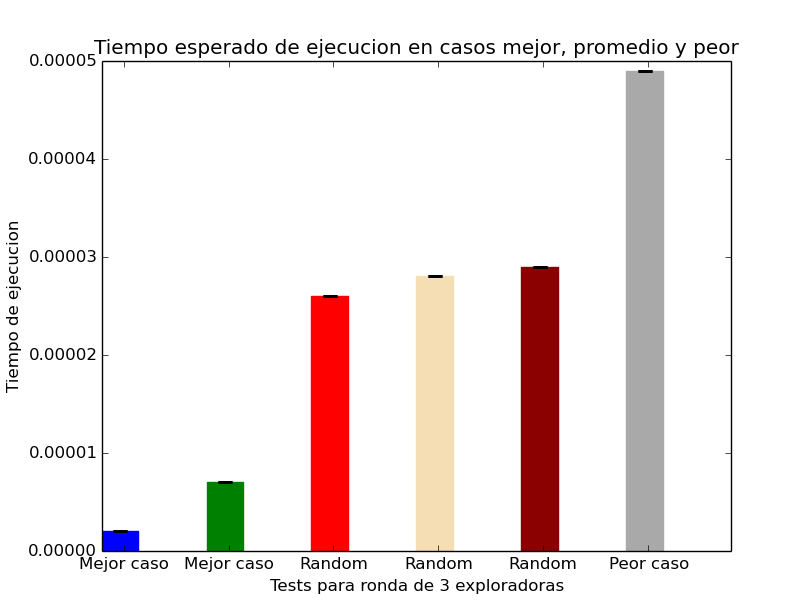
\includegraphics[scale=0.4]{tiemposE3}
        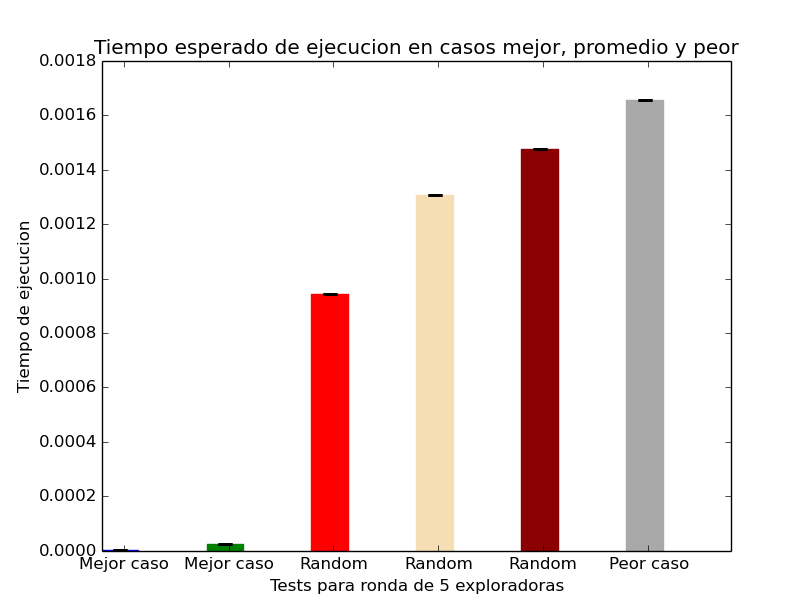
\includegraphics[scale=0.4]{tiemposE5}
      \end{figure}
      \begin{figure}[H]
        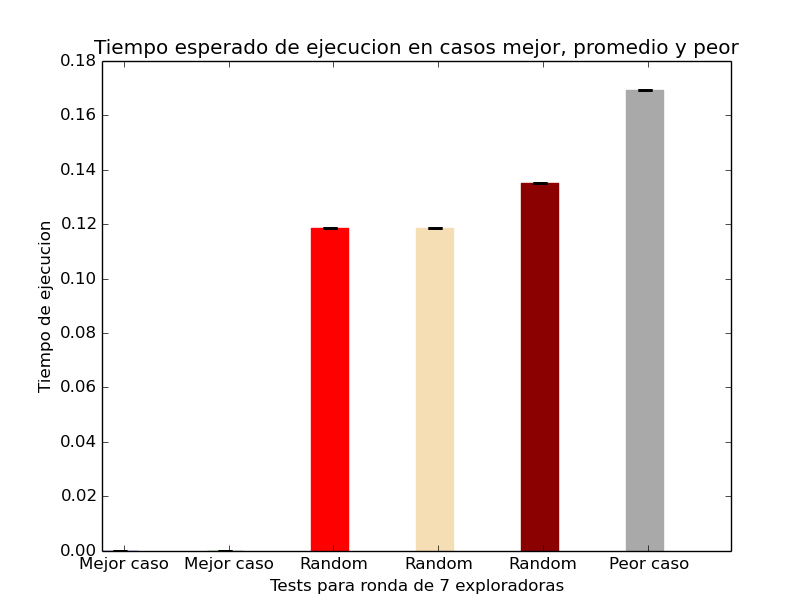
\includegraphics[scale=0.4]{tiemposE7}
        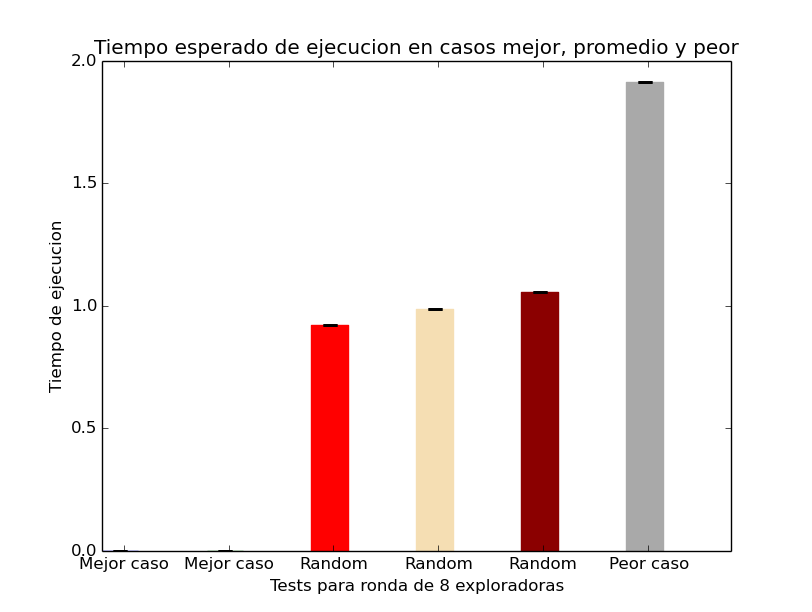
\includegraphics[scale=0.4]{tiemposE8}
      \end{figure}

Por cada tamaño calculamos el tiempo para los dos mejores casos, el de más a la izquierda cuando el conjunto de amistades es 
nulo, y a su derecha cuando el conjunto de amistades es el más grande posible. A mayor tamaño del grupo de exploradoras los mejores casos 
se mantienen casi iguales, mientras que los otros casos crecen de manera abrupta. Esto sucede ya que la complejidad de los mejores casos es 
cuadratica en $e$, mientras que los otros son factoriales. Podemos notar como en los casos $e$ = 3 y $e$ = 5 hay una diferencia de rendimiento entre los 
mejores casos. Esto se da porque el segundo tiene que almacenar todo el conjunto de amistades en memoria, lo cual hace que tenga un heap mayor 
que el primero. Por ende, esa pequeña diferencia de rendimiento.

Para las muestras indicadas como random realizamos tests sin ninguna intencionalidad. Para generarlos establecimos un conjunto de 
exploradoras fijo y luego generamos de manera pseudoaleatoria el conjunto de amistades. Generamos un número random 
utilizando la función \textbf{rand\_r} y luego le aplicamos al resultado módulo tamaño de la ronda. Así obtuvimos una exploradora al azar. 
Repetimos el procedimiento con la segunda elección hasta que sea distinta de la primera. Iteramos este procedimiento $\frac{e*(e-1)}{2}$
ya que es el la cantidad máxima de posibles amistades.

Para evaluar el peor caso hicimos tests donde todas las exploradoras eran amigas entre sí, excepto por un par. 

Como aclaramos previamente que una vez fijada la cantidad de exploradoras la complejidad temporal del algoritmo 
depende exclusivamente del cardinal del conjunto de amistades, mostramos los siguientes datos:
\begin{itemize}
  \item Para todos los gráficos el cardinal del conjunto de amistades en los mejores casos son 0 y $\frac{e*(e-1)}{2}$
  \item Para el test con 3 exploradoras el cardinal de amistades es:
    \begin{itemize}
      \item Rojo: 1  \ \ \ \ \ \ \inlineitem Rosa : 1 \ \ \ \ \ \  \inlineitem Marrón : 1  \ \ \ \ \ \ \inlineitem Gris  : 2
    \end{itemize}
  \item Para el test con 5 exploradoras el cardinal de amistades es:
    \begin{itemize}
      \item Rojo: 5  \ \ \ \ \ \ \inlineitem Rosa : 7 \ \ \ \ \ \  \inlineitem Marrón : 8  \ \ \ \ \ \ \inlineitem Gris  : 10
    \end{itemize}
  \item Para el test con 7 exploradoras el cardinal de amistades es:
    \begin{itemize}
      \item Rojo: 14  \ \ \ \ \ \inlineitem Rosa : 14  \ \ \ \ \  \inlineitem Marrón : 16  \ \ \ \ \ \ \inlineitem Gris  : 21
    \end{itemize}
  \item Para el test con 8 exploradoras el cardinal de amistades es:
    \begin{itemize}
      \item Rojo : 13 \ \ \ \ \ \inlineitem Rosa : 14  \ \ \ \ \  \inlineitem Marrón : 15  \ \ \ \ \ \ \inlineitem Gris  : 28
    \end{itemize}
\end{itemize}

Por ende, una vez fijada la cantidad de exploradoras, podemos observar cómo el tiempo de ejecución del algoritmo 
difiere en base a la cantidad de amistades. 

Como nuestro algoritmo utiliza la técnica de backtracking, la cual consiste en explorar todas las posibles 
soluciones, consideramos utilizar una poda para mejorar el rendimiento. Como el algoritmo pide 
encontrar la ronda que, además de que cumpla la condición de las distancias, también sea la menor lexicográficamente 
se puede utilizar esta información para acotar el espacio de posibles soluciones. En el ejercicio modelamos 
una ronda y lo que nos interesa como resultado es la distancia relativa entre cada amiga, no su posición en la ronda. 
Con sólo explorar las posibles permutaciones que comienzan con la exploradora que es la menor lexicográficamente 
de todo el conjunto es suficiente. Esto sucede porque dada cualquier ronda que no empiece con la menor exploradora, 
se la puede reacomodar a través de rotaciones simples entre las exploradoras contiguas, hasta llegar a una ronda 
cuya distancia entre todas es la misma (ya que no modificamos sus distancias relativas) y es menor lexicográficamente.

A continuación mostramos de manera gráfica la comparacion entre los peores tiempos del algoritmo con distintos tamaños de exploradoras.
A la izquierda se encuentra el tiempo estimado del peor caso común, y a la derecha el peor caso utilizando la poda:

      \begin{figure}[h]
        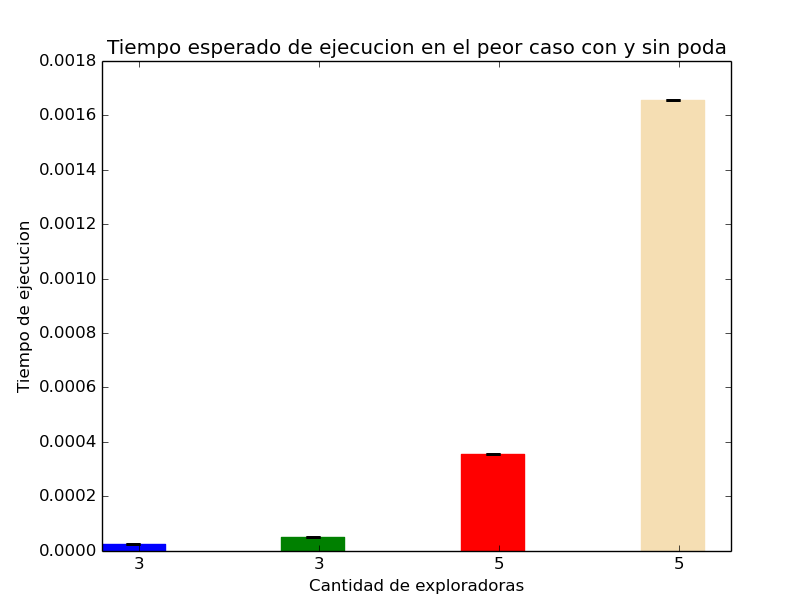
\includegraphics[scale=0.4]{tiempoE3P}
        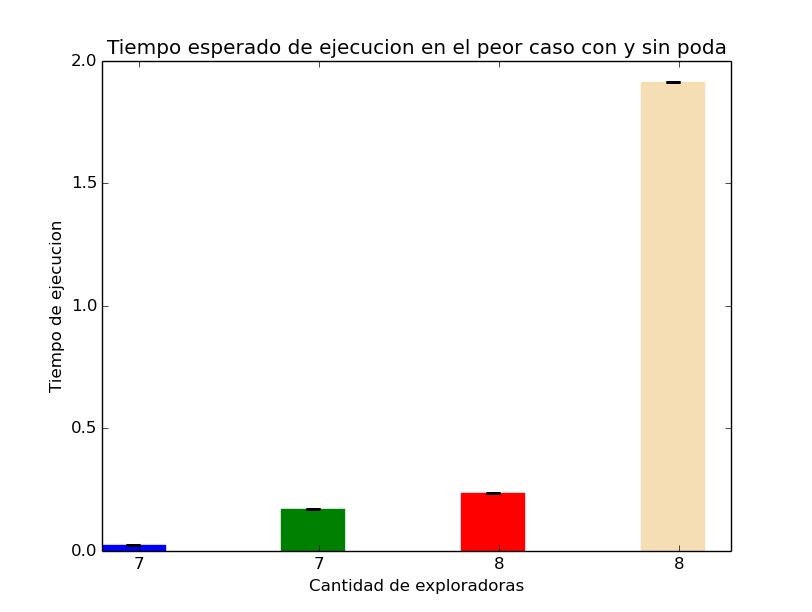
\includegraphics[scale=0.4]{tiempoE7P}
      \end{figure}

Podemos notar como a medida que crece el tamaño del conjunto de exploradoras, la diferencia de rendimiento entre utilizar o no la poda 
es cada vez mayor.


























\section{Tests}


\subsection{El Telégrafo}

Para generar los tests usados en el Ejercicio 1 se procedió de diversas maneras:

\begin{enumerate}

\item[Mejor Caso:] Se generó un intervalo de $n$ ciudades (sin contar la capital) con una distancia de 1 km entre cada una, es decir que si quiero generar un intervalo de 10 ciudades, se generará el intervalo: 0 1 2 3 4 5 6 7 8 9 10.

Se proveen 0 km de cable, de forma que se asegure que se itera por el intervalo una sola vez (moviendo ambos índices al mismo tiempo en cada iteración).

\item[Caso al Azar:] Se genera un intervalo tomando un número aleatorio dentro un rango definido y luego se suma dicho número a un acumulador que comienza en 0, dicho acumulador es, en cada iteración, una nueva ciudad.

De esta manera, se consigue generar ciudades separadas entre sí por una distancia al azar.

Se provee un número al azar de km de cable, entre 0 y la distancia entre la última ciudad generada y la capital.

\item[Peor Caso:] Se toma el mismo caso de test generado por el generador de tests aleatorios, pero se modifica la distancia de la última ciudad, para que sea el doble de la cantidad de cable provista.

Como consecuencia de esto, se fuerza al índice $i$, que es aquel que, por lo general, no requiere recorrer toda la lista, a terminar de recorrerla, efectivamente aumentando el tiempo de iteración a O(2n), en contraste con el tiempo de iteración O(n) del mejor caso.

\end{enumerate}


\subsection{A Medias}


Cada línea del archivo representa un caso de test.

El input de la línea 2 es un caso en el cual el flujo del programa recorre todos los casos posibles de las instrucciones de control, es decir, recorre todas las ramas de todos los $if$, ejecutando así todas las líneas del código.

El input de la línea 3 es un mejor caso para el algoritmo, que inserta un elemento en un $heap$ distinto cada vez.

El input de la línea 4 es un peor caso, en el que todas las inserciones se realizan en el mismo heap, y es necesario rebalancear uno todas las iteraciones, y el otro una vez cada dos elementos insertados.

\section{Apéndice}

\subsection{Codigo fuente}

\newpage
\subsubsection{A medias}
\lstinputlisting[language=Octave]{mediana.cpp.src}
\newpage

\end{document}
